\documentclass[11pt]{article}
\usepackage[margin=1in]{geometry}
\usepackage{graphicx}
\usepackage[font={small, it}]{caption}
\usepackage{matlab-prettifier}
\usepackage{listings}
\usepackage{keystroke}
\usepackage{menukeys}
\usepackage{amsthm}
\usepackage{subfigure}
\lstset{ %
language=Matlab,                % choose the language of the code
basicstyle=\footnotesize,       % the size of the fonts that are used for the code
numbers=left,                   % where to put the line-numbers
numberstyle=\footnotesize,      % the size of the fonts that are used for the line-numbers
stepnumber=1,                   % the step between two line-numbers. If it is 1 each line will be numbered
numbersep=5pt,                  % how far the line-numbers are from the code
backgroundcolor=\color{white},  % choose the background color. You must add \usepackage{color}
showspaces=false,               % show spaces adding particular underscores
showstringspaces=false,         % underline spaces within strings
showtabs=false,                 % show tabs within strings adding particular underscores
frame=single,           % adds a frame around the code
tabsize=2,          % sets default tabsize to 2 spaces
captionpos=b,           % sets the caption-position to bottom
breaklines=true,        % sets automatic line breaking
breakatwhitespace=false,    % sets if automatic breaks should only happen at whitespace
escapeinside={\%*}{*)}          % if you want to add a comment within your code
}

% Define an Example environment
\theoremstyle{definition}
\newtheorem{exmp}{Example}[section]

\usepackage{hyperref}		% Enables hyperlinks via "\hyperref{}" and "\href{}{}" and "\url{}"
\usepackage{soul} 
\newcommand{\myhref}[2]{\textcolor{blue}{\href{#1}{\ul{#2}}}}

% Title information
\author{Enrique P. Blair, Ph.D.}
\title{An Introduction to Object-oriented Programming in MATLAB}

% ============================================
% ============================================
% ============================================
% ============================================
% ============================================
% ============================================
\begin{document}
% ============================================
% ============================================
% ============================================
% ============================================
% ============================================
% ============================================

\maketitle

\tableofcontents

\clearpage

% !TEX root = MATLAB_OOP_Blair.tex

% ============================================================
% ============================================================
% ============================================================
\section{Introduction to Object-oriented Programming in MATLAB}
% ============================================================
% ============================================================
% ============================================================

% ============================================================
% ============================================================
\subsection{Object-oriented Programming}
% ============================================================
% ============================================================

Object-oriented programming (OOP) is a powerful approach to writing complex software suites that handle non-trivial tasks and calculations. In OOP, the programmer defines \textbf{classes}, which are user-defined, composite data types with associated functions known as \textbf{methods}. methods define how an end-user interacts with \textbf{objects}, which are \textbf{instances} of a class.  Thus, programming which involves the use of classes is called object-oriented programming (OOP).

% ============================================================
% ============================================================
\subsection{Data Types}
% ============================================================
% ============================================================

\subsubsection{Elementary Data Types}
In MATLAB, basic or ``elementary'' data types include \texttt{double} (double-precision floating-point data) and \texttt{char} (characters). Numbers in MATLAB are stored in memory as data of type \texttt{double}. MATLAB also handles arrays of \texttt{double}s, which also are said to be of type \texttt{double}.

Additionally, MATLAB has variables of type \texttt{char}, which store lowercase letters (\texttt{'a'}-\texttt{'z'}), upper-case letters (\texttt{'A'}-\texttt{'Z'}), numerals (\texttt{'0'}-\texttt{'9'}), and myriad other special characters. \textbf{Strings} are arrays (typically, row vectors) of \texttt{char}s, and are themselves considered to be of type \texttt{char}.

\subsubsection{Arrays}

Arrays store multiple values of the same data type. Each individual value in an array is called an \textbf{element}. In MATLAB, arrays are formed by concatenating elements within brackets (\texttt{[} and \texttt{]}). Horizontal concatenation is achieved by grouping elements within brackets but delimiting (separating) them either by commas (\texttt{,}) or by white space. Vertical concatenation is achieved by delimiting constituents by a semicolon (\texttt{;}). Examples of this are given in the command-line sample below:
% vvv------------------------------------------------------------vvv
\begin{lstlisting}[style=Matlab-editor, caption={The Command Window input and output demonstrates horizontal concatenation and vertical concatenation. Concatenation is accomplished using brackets \texttt{[} and \texttt{]}. Elements of a horizontal concatenation are separated by whites space or commas (\texttt{,}); and elements of a vertical concatenation are specified using a semicolon (\texttt{;}).}, label={lst:ConcatenationCommandWindow}]
 >> A = [1 2 3]; B = [4 5 6]; C = [A B]

C =

     1     2     3     4     5     6

>> D = [A; B]

D =

     1     2     3
     4     5     6
\end{lstlisting}
 % ^^^------------------------------------------------------------^^^
In line 1 of Listing \ref{lst:ConcatenationCommandWindow}, we define \texttt{A} as the horizontal concatenation of 1, 2, and 3; and \texttt{B} as the horizontal concatenation of 4, 5, and 6. Then, \texttt{C} is formed by horizontally concatenating \texttt{A} and \texttt{B}. The output of line 1 is shown in lines 3-5. Finally, in line 7, \texttt{D} is formed by vertically concatenating \texttt{A} and \texttt{B}, with output on lines 9-12. Similar concatenation may be achieved using strings. Similar concatenations may be done using data of type \texttt{char}. To form an array, all elements have the same data type and the same size in memory.

MATLAB also has another type, known as a \texttt{cell} (short for ``cell array''), in which each element may be of a different type or of different sizes in memory. MATLAB \texttt{double} arrays of different sizes, \texttt{char} arrays different sizes, and even other \texttt{cell}s may be elements of the same \texttt{cell}.

% ============================================================
% ============================================================
\subsubsection{Structures}
% ============================================================
% ============================================================

MATLAB allows the formation of \textbf{data structures} (or simply ``structures'' for short; and \texttt{struct}s in MATLAB). A structure is a composite variable comprised of multiple pieces of data. MATLAB \texttt{struct}s are very flexible, as a \texttt{struct} may contain data of elementary data types, arrays, cell arrays, other \texttt{structs}, or even more complex and elaborate data types (classes). The constituent data associated with a \texttt{struct} are called \textbf{fields}. We use ``dot syntax'' to define, assign, and reference the fields of a \texttt{struct}. For example, the following input (line 1) defines a new \texttt{struct}, \texttt{S}, with one field, \texttt{a}, and the \texttt{double} 7 is stored in the field \texttt{S.a}. Then, in line 9, a new field, \texttt{b} is added to \texttt{S}, and \texttt{char} array \texttt{'life'} is stored in \texttt{S.b}.
% vvv------------------------------------------------------------vvv
\begin{lstlisting}[style=Matlab-editor]
>> S.a = 7

S = 

  struct with fields:

    a: 7

>> S.b = 'life'

S = 

  struct with fields:

    a: 7
    b: 'life'
>> y = S.a + 5

y =

    12

>> disp(['The word is: ', S.b])
The word is: life
\end{lstlisting}
% ^^^------------------------------------------------------------^^^
Lines 17 and 23 show how the values stored in \texttt{S.a} and \texttt{S.b} may be referenced and used in further calculations.

Additionally, a \texttt{struct} may be formed by specifying field-value pairs in the \texttt{struct()} command:
% vvv------------------------------------------------------------vvv
\begin{lstlisting}[style=Matlab-editor]
>> R = struct('a', 7, 'b', 'life')

R = 

  struct with fields:

    a: 7
    b: 'life'

>> 
\end{lstlisting}
% ^^^------------------------------------------------------------^^^


\texttt{struct}s are particularly useful for storing various pieces of information associated with one system or event in real life. For example, conditions (location, temperature, pressure, time, etc.) and data measurements for a particular experiment may be stored in the same \texttt{struct}. Or, you might want a \texttt{struct} to store the name, phone number, e-mail address, website and other information for a particular friend, relative, or contact. Then, a collection of such \texttt{struct}s can constitute an address book.

% ============================================================
% ============================================================
\subsection{Functions}
% ============================================================
% ============================================================
Functions are an important element of OOP, so we discuss them here only briefly. In contrast, students in computer-related disciplines may take an entire course on functional programming.

Functions enable code to be modular. A well-written function does a specific task or returns an output based on a set of inputs. The details of the function may be transparent to the user, who can repeatedly call a function without repeatedly copying and pasting the code that underlies the function. This makes the user's code clearer and more understandable. Additionally, if the function requires modification, the implementation of the function may be modified without changing the user's interface of the function.

% ============================================================
\subsection{Pre-defined Functions}
% ============================================================
MATLAB has numerous pre-defined functions. Here, we discuss a few functions that will be used in following sections of this document.

% ============================================================
\subsubsection{Mathematical Functions}
% ============================================================
MATLAB has numerous mathematical functions for performing calculations, including \texttt{sin()}, \texttt{cos()}, \texttt{real()}, \texttt{imag()}, \texttt{sinc()}, \texttt{exp()}, and so many more.

% ============================================================
\subsubsection{The \texttt{class()} Function}
% ============================================================
This returns the data type of a variable. In the following code, we define a few variables of different types, and then we use the \texttt{class} function to identify their type.
% vvv------------------------------------------------------------vvv
\begin{lstlisting}[style=Matlab-editor]
>> a = 5;
>> class(a)

ans =

    'double'

>> class(pi)

ans =

    'double'

>> b = rand(3, 4);
>> class(b)

ans =

    'double'

>> class('s')

ans =

    'char'

>> class('cat')

ans =

    'char'
    
>> friend1.name = 'Alice'; friend1.age = 23; class(friend1)

ans =

    'struct'
\end{lstlisting}
% ^^^------------------------------------------------------------^^^
Here, we see that numbers and arrays of numbers are of class (type) \texttt{double}, and characters and arrays of characters are of class \texttt{char}.

% ============================================================
\subsubsection{The \texttt{length()} Function}
% ============================================================
The command \texttt{length(X)} returns the number of elements in the array \texttt{X}. Some examples of this are shown in the following listing:
% vvv------------------------------------------------------------vvv
\begin{lstlisting}[style=Matlab-editor]
>> A = 1:7

A =

     1     2     3     4     5     6     7

>> length(A)

ans =

     7

>> B = (12:16)'

B =

    12
    13
    14
    15
    16

>> length(B)

ans =

     5
\end{lstlisting}
% ^^^------------------------------------------------------------^^^
For a matrix \texttt{X}, the command \texttt{length(X)} returns the size of the largest dimension of \texttt{X}:
% vvv------------------------------------------------------------vvv
\begin{lstlisting}[style=Matlab-editor]
>> C = rand(3,4)

C =

    0.6541    0.4505    0.9133    0.5383
    0.6892    0.0838    0.1524    0.9961
    0.7482    0.2290    0.8258    0.0782

>> length(C)

ans =

     4

>> D = rand(4,3)

D =

    0.4427    0.7749    0.3998
    0.1067    0.8173    0.2599
    0.9619    0.8687    0.8001
    0.0046    0.0844    0.4314

>> length(D)

ans =

     4
\end{lstlisting}
% ^^^------------------------------------------------------------^^^
This is equivalent to using the command \texttt{max(size(X))}.


% ============================================================
\subsubsection{The \texttt{disp()} Function}
% ============================================================
The \texttt{disp()} function writes a string to the MATLAB Command Window output, as shown in the following listing:
% vvv------------------------------------------------------------vvv
\begin{lstlisting}[style=Matlab-editor]
>> some_str = 'hello';
>> disp(some_str)
hello
\end{lstlisting}
% ^^^------------------------------------------------------------^^^

% ============================================================
\subsubsection{The \texttt{num2str()} Function}
% ============================================================
The \texttt{num2str(x, formatStr)} converts a number (\texttt{double}) to a \texttt{char} string, with options specified using the string \texttt{formatStr}.

If we wish to display  the value of a number using \texttt{disp()}, we must convert it to a string first. This may be done using \texttt{(num2str()}, for example:
% vvv------------------------------------------------------------vvv
\begin{lstlisting}[style=Matlab-editor]
>> x = 9;
>> disp(['x = ', num2str(x)])
x = 9
\end{lstlisting}
% ^^^------------------------------------------------------------^^^
Since \texttt{disp()} receives only one string input argument, we horizontally concatenate the two strings \texttt{'x = '} and \texttt{num2str(x)} into one using horizontal concatenation.

% ============================================================
\subsubsection{Obtaining Time Intervals using \texttt{tic} and \texttt{toc}}
% ============================================================

Have you ever wished that you can use a stopwatch in MATLAB? This can allow you to determine how long some code will take, like starting a stopwatch when a runner leaves the starting line and stopping it when she crosses the 400-m mark. This could also allow you to execute a \texttt{while} loop as long as elapsed time is within some limit.

Time intervals may be measured using the \texttt{tic} and \texttt{toc} commands. When you wish to start the time, use \texttt{tic}. A subsequent \texttt{toc} stops the timer and returns the time interval measurement; or you can measure a time interval and make a count-down timer. For example:
% vvv------------------------------------------------------------vvv
\begin{lstlisting}[style=Matlab-editor]
>> tic; % like starting a stopwatch
pause(0.25); % insert a pause to simulate some commands run
time_elapsed = toc % ends the timer and reports the time elapsed

time_elapsed =

    0.2555

>> 
\end{lstlisting}
% ^^^------------------------------------------------------------^^^
Using a variable, such as \texttt{x = tic}, establishes \texttt{x} as a time marker. When supplied as an input to the \texttt{toc} command, \texttt{toc} returns time elapsed since \texttt{x} was defined. Thus, multiple reference points may be used in a calculation. For example, code like this may be used:
% vvv------------------------------------------------------------vvv
\begin{lstlisting}[style=Matlab-editor]
start_time = tic; % interval start time reference
pause(0.25); % insert a pause to simulate some commands run
first_interval = toc(start_time); % measure first time interval
mid_time = tic; % adds a second reference, mid_time
pause(0.75);  % insert a pause to simulate some commands run
end_interval = toc(mid_time); % measure time since mid_time
total_time = toc(start_time); % measure time since first_time
disp(sprintf('First interval: %5.3f s', first_interval) )
disp(sprintf('Second interval: %5.3f s', end_interval))
disp(sprintf('Total duration: %5.3f s', total_time))
\end{lstlisting}
% ^^^------------------------------------------------------------^^^
The output would be something like this:
% vvv------------------------------------------------------------vvv
\begin{lstlisting}[style=Matlab-editor]
First interval: 0.257 s
Second interval: 0.755 s
Total duration: 1.016 s
\end{lstlisting}
% ^^^------------------------------------------------------------^^^

To see more demonstrations of \texttt{tic} and \texttt{toc}, see \myhref{https://youtu.be/Bpsuf-wE6eY}{this video}.

% ============================================================
\subsection{User-defined Functions}
% ============================================================
A MATLAB function is typically defined in a text file with the extension \texttt{*.m}. Here are some salient features of a function definition file.

\begin{enumerate}
\item The name of the \texttt{*.m} file must match the function name exactly (MATLAB is case-sensitive).
\item The file begins with the keyword \texttt{function}, followed by the name of the function. This first line of the function is called the \textit{header}, and it specifies how the user interacts with the function. The syntax of the function header (with end) is given below:
% vvv------------------------------------------------------------vvv
\begin{lstlisting}[style=Matlab-editor]
function [out1, out2] = functionName( in1, in2, in3 )
	statements
end
\end{lstlisting}
% ^^^------------------------------------------------------------^^^
Here, the function \texttt{functionName} is a three-input, two-output function.
\item The file ends with the keyword \texttt{end}.
\item The \textit{body} consists of the statements that specify the function implementation. The body is written between the header and the closing \texttt{end} statement. There may be only very few statements in the body, or several hundreds or even thousands of lines of code in a function body.
\item The function header defines the inputs required by the function, as well as the outputs provided by the function.
\begin{enumerate}
\item Functions may be designed with no input or output, or few inputs and outputs, or even variable inputs and outputs.
\item Functional inputs and outputs are called \textbf{arguments} or \textbf{parameters}. The parameters defined in the header are to be used within the function body.
\end{enumerate}
\item Commented lines of code immediately following the header provide function help documentation. When you type \texttt{help functionName} in the command line, the function help you defined appears in the command line.
\end{enumerate}

% ============================================================
% ============================================================
\exmp{Example}
Write and test a function that calculates $f(x,y,z)$, where $$f(x,y,z) = x + y^2 + z^3 .$$

\noindent \underline{Solution}.
Here, there are three input parameters: $x$, $y$, and $z$; and one output parameter $f$. Thus, we can accomplish this by writing the following function and saving it in the text file \texttt{f\_function.m} of Listing \ref{lst:function_def}:
% vvv------------------------------------------------------------vvv
\begin{lstlisting}[style=Matlab-editor, caption={The code of the function-definition file \texttt{f\_function.m}.}, label={lst:function_def}]
function f = f_function(x, y, z)
%f_function calculates f(x, y, z), where
%   f(x,y,z) = x + y^2 + z^3
%
% By E.P. Blair
% Baylor University
%
f = x + y^2 + z^3;
end
\end{lstlisting}
% ^^^------------------------------------------------------------^^^

To test \texttt{f\_function.m}, we can write a \textit{testbed} script, or we can simply try it in the command line. A testbed script is one which invokes a function of interest in order to test whether it performs as designed. Here, however, we simply test \texttt{f\_function()} in the MATLAB command line:
% vvv------------------------------------------------------------vvv
\begin{lstlisting}[style=Matlab-editor, caption={MATLAB Command Window input invoking \texttt{f\_function()}, along with the resulting output.}, label={lst:CmdWinTest_f_function}]
>> f = f_function(1, 1, 1)

f =

     3

>> f = f_function(1, 2, 3)

f =

    32
\end{lstlisting}
% ^^^------------------------------------------------------------^^^
Line 1 of Listing \ref{lst:CmdWinTest_f_function} invokes \texttt{f\_function()} with $x=y=z=1$, which returned the correct result: $f(1,1,1) = 1 + 1^2 +1^3 = 3$. This matches the output of lines 3-5. The next invocation of \texttt{f\_function()} correctly evaluated $f(1,2,3) = 1 + 2^2 +3^3 = 1 + 4 + 27 = 32$, shown in the result of lines 9-11. Thus, \texttt{f\_function()} appears to work correctly.

Functions may also take data of type \texttt{char}, \texttt{cell}, \texttt{struct}, or even objects of classes as input. Outputs may be of the same types.



% ============================================================
\subsubsection{The \texttt{varargin} Keyword}
% ============================================================
The key word \texttt{varargin} may be used in a function header to allow a variable number of input arguments. For example, in the function definition below, inputs \texttt{in1}, \texttt{in2}, and \texttt{in3} are mandatory, but \texttt{varargin} allows for zero or more additional input arguments.
% vvv------------------------------------------------------------vvv
\begin{lstlisting}[style=Matlab-editor]
function [out1, out2] = functionName( in1, in2, in3, varargin)
	statements
end
\end{lstlisting}
% ^^^------------------------------------------------------------^^^
Thus, through the flexibility afforded by \texttt{varargin}, the following invocations of \texttt{functionName} all are valid:
% vvv------------------------------------------------------------vvv
\begin{lstlisting}[style=Matlab-editor]
[a, b] = functionName( x, y, z );

[c, d] = functionName( x, y, z, e );

[g, h] = functionName( x, y, z, e, j, k );
\end{lstlisting}
% ^^^------------------------------------------------------------^^^
Of course, we must design the body of \texttt{functionName()} to correctly support the various invocations.

% ============================================================
\subsubsection{The \texttt{nargin} Function}
% ============================================================
MATLAB has a special function named \texttt{nargin}. When invoked inside another function, \texttt{nargin} returns the number of input arguments specified in an invocation of the function of interest. This is particularly useful when that function is designed to support variable input arguments using \texttt{varargin}. Here, we may use \texttt{nargin} with some logical control structure, such as \texttt{if}-\texttt{else} or \texttt{switch}-\texttt{case}.

You may already have used \texttt{varargin} this without knowing it if you have used the \texttt{plot()} command:
% vvv------------------------------------------------------------vvv
\begin{lstlisting}[style=Matlab-editor]
x = linspace(0, 1, 101);
y = sin(2*pi*x);
figure;
plot(x, y); % generates a default plot
figure % new figure
plot(x, abs(y), 'LineWidth', 2', 'LineStyle', '--'); % new plot, this time with options
\end{lstlisting}
% ^^^------------------------------------------------------------^^^
Notice that we use the same \texttt{plot()} function, but with a different number of arguments. The key to doing this is \texttt{varargin}, and now that key is in your hand!

For example, here is a function that allows a user to calculate values of a quadratic or a cubic expression:
% vvv------------------------------------------------------------vvv
\begin{lstlisting}[style=Matlab-editor]
function y = calc_poly(x, a, b, c, varargin)
%CALC_POLY calculates the value of a quadratic, cubic or quartic
%        expressions.
%
% SYNTAX
% ======
%   y = calc_poly(x, a, b, c ) evaluates the value of the quadratic
%       expression a*x^2 + b*x + c
%
%   y = calc_poly(x, a, b, c, d ) evaluates the value of the cubic
%       expression a*x^3 + b*x^2 + c*x + d
%
%   y = calc_poly(x, a, b, c, d, f ) evaluates the value of the
%        quartic expression a*x^4 + b*x^3 + c*x^2 + d*x + f
%
% By. E.P. Blair
% Baylor University
% 2021.04.17

switch nargin % number of input arguments
    case 4 % quadratic
        y = a*x.^2 + b*x + c;
        
    case 5  % cubic
        d = varargin{1};
        y = a*x.^3 + b*x.^2 + c*x + d;
        
    case 6  % quartic
        d = varargin{1};
        f = varargin{2};
        y = a*x.^4 + b*x.^3 + c*x.^2 + d*x + f;

    otherwise
        error(['calc_poly: invalid number (', num2str(nargin), ...
            ') of input arguments.'])

end
\end{lstlisting}
% ^^^------------------------------------------------------------^^^




% ============================================================
% ============================================================
\subsection{Classes}
% ============================================================
% ============================================================

\subsubsection{Beyond Structures}
Sometimes, simply storing information in structures is not enough. In these cases, it is desirable to perform manipulations on the various groups of information, or model the effects of particular events on the items represented by structures. In these cases, it is powerfully helpful to define \textbf{classes}. Classes extend the capability of \texttt{struct}s by defining a standard set of fields, called \textbf{properties}, and by defining an associated set of class \textbf{methods}. A particular instance or extended \texttt{struct} of a class is called an \textbf{object}. We can think of an object as a variable of a custom-data type (the class). Methods\textemdash sometimes called \textit{behaviors} in other programming languages \textemdash are a set of functions that are used to extract information from or manipulate objects.

\subsubsection{Motivation for Classes}
One example where classes might be useful is in an online gaming system. Here, we might want a class called \texttt{Avatar} (we will use the convention in which we capitalize the name of a user-defined class to distinguish it from MATLAB's own pre-defined classes). For each individual player, an object of class \texttt{Avatar} may store the user's real name, handle, level, experience points, maximum vitality, and health. Then, \texttt{Avatar} class methods can define operations on objects such as \texttt{gainXP()} to add to a player's experience points, \texttt{levelUp()} to implement an irreversible milestone in the development of the player's avatar, and \texttt{attack()} to model one player's attack on another player, which may detract from the health of the target of the attack. One can imagine myriad other methods that might be desirable in a complex gaming system.

Another example in which classes may be useful is in the design of a software system that tracks an individual's investments. Investments may be in stocks and mutual funds. We might wish to make an \texttt{Asset} class that stores in its member data an asset name, a symbol, and based on a list of transactions, can calculate the worth of that particular holding. A transaction can be represented by objects of a \texttt{Transaction} class, which stores information about the transaction date, the type of transaction(open, buy, sell, split, dividend, short, close out, etc.), the number of shares transacted, the price per share, and any transaction fees. A particular \texttt{Asset} object may include a list of transactions. With the list of transactions and up-to-date information about share price, an \texttt{Asset} class method, say, \texttt{calculateValue()}, may be used to calculate the worth of the holding. Then, a \texttt{Portfolio} class may be designed to contain multiple \texttt{Asset} objects. The \texttt{Portfolio} class, then, is called a \textbf{container} class for \texttt{Asset} objects.

\subsubsection{The Advantages of Classes}

One might think that classes add complexity to computer programs. Indeed, classes and OOP allow vast complexity to be handled in a clean and logical manner. Some of the benefits of using classes:

\begin{enumerate}
\item Encapsulation. Many lines of code\textemdash think hundreds or thousands\textemdash required to implement an operation on an object may be cleanly invoked with a simple call to a method function. Also, if we must modify the method, it can be done once in the class definition. This ``under-the-hood'' modification may be transparent to a user, who can invoke the modified function using the same syntax as before, but with the benefits of an improved method.

\item Understandability. With well-chosen, smartly-defined methods, OOP adds great understandability. Complex tasks can be executed by invoking aptly-named methods.

\item Hierarchical methods. The user can invoke a method a container-class object, and the container-class method can automatically invoke a method of the objects contained therein. For example, a \texttt{Portfolio}-class method \texttt{calculateValue()} can invoke the \texttt{calculateValue()} for each asset therein. It can gather the returned values and sum them, to report the value of the investment portfolio it represents. This complex method is transparent to the user, who simply queries the \texttt{Portfolio}-class object for its value.
\end{enumerate}

% !TEX root = MATLAB_OOP_Blair.tex

% ============================================================
% ============================================================
% ============================================================
\section{Built-in Classes}
% ============================================================
% ============================================================
% ============================================================

We will gain some experience with classes with MATLAB's built-in classes. A class defines a composite data type. When we define \texttt{n = 71.9}, we say that \texttt{n} is a variable of type \texttt{double}. Similarly, a variable belonging to some class is called an \textbf{object}. You'll also hear it said that we \textit{instantiate} an object of a certain class, or that some object is an instance of some class.  If we were to write an analogy, we might write \texttt{type:variable::class:object}. We can say that a class is a generalization of the concept of a variable.

Like a \texttt{struct}, an object may have multiple elementary data types embedded in it. In a \texttt{struct}, the constituent data elements are called ``fields,'' but in an object the constituent data elements are called ``properties.''

% ============================================================
% ============================================================
\subsection{The \texttt{datetime} Class}
% ============================================================
% ============================================================
The \texttt{datetime} class is provided to allow users to create and manipulate dates.

% ============================================================
\subsubsection{Creating a New \texttt{datetime} Object}
% ============================================================

We can instantiate a \texttt{datetime} object, \texttt{x}, as follows:
% vvv------------------------------------------------------------vvv
\begin{lstlisting}[style=Matlab-editor, caption={This input to the MATLAB Command Window input uses the \texttt{datetime()} constructor method to instantiate a \texttt{datetime} object, \texttt{x}.}]
>> x = datetime('now')

x = 

  datetime

   17-Apr-2021 19:44:34

>> class(x)

ans =

    'datetime'
\end{lstlisting}
% ^^^------------------------------------------------------------^^^
MATLAB automatically reports that this is a \texttt{datetime} object, and the \texttt{class} function is in agreement with this.

% ============================================================
\subsubsection{Properties}
% ============================================================
Building on the previous code block, we can then use the \texttt{properties()} function to discover what properties the object \texttt{x} has. Then, we can reference those properties using the dot syntax:
% vvv------------------------------------------------------------vvv
\begin{lstlisting}[style=Matlab-editor, caption={The \texttt{properties()} function lists the accessible properties of the \texttt{x} object.}]
>> properties(x)

Properties for class datetime:

    Format
    TimeZone
    Year
    Month
    Day
    Hour
    Minute
    Second
    
>> x.Year

ans =

        2021

>> disp(['Month: ', num2str(x.Month)])
Month: 4
\end{lstlisting}
% ^^^------------------------------------------------------------^^^


% ============================================================
\subsubsection{Method Functions}
% ============================================================

Any function associated with a class is called a \textbf{method function}, or simply a ``method.'' Methods define how objects can be used and manipulated, and how data contained in functions can be accessed.

The \texttt{datetime} function is actually a special method called a \textbf{constructor method}. This defines how a new object is instantiated for the class. In the previous code block, we use the string \texttt{'now'} as an input to the constructor \texttt{datetime}. This caused \texttt{datetime} to obtain the current computer clock time and form a \texttt{datetime} object. The \texttt{datetime} constructor may also be used to create a \texttt{datetime} object for a specific day:
% vvv------------------------------------------------------------vvv
\begin{lstlisting}[style=Matlab-editor, caption={A \texttt{datetime} object is created to represent October 5, 2016 as a birthday.}]
>> bday = datetime(2016, 10, 5)

bday = 

  datetime

   05-Oct-2016

>> age = between(bday, datetime('now'))

age = 

  calendarDuration

   4y 6mo 13d 0h 24m 30.366s

\end{lstlisting}
% ^^^------------------------------------------------------------^^^
 You can use \texttt{help datetime} to discover other ways to use the \texttt{datetime} constructor.

Other methods can be defined to access, display or manipulate the data in an object. For example, \texttt{between} is a \texttt{datetime} function designed to find the duration between two \texttt{datetime} objects, as in lines 9-15 of the above listing.



% ============================================================
% ============================================================
\subsection{MATLAB Graphics Classes}
% ============================================================
% ============================================================

If you've used MATLAB graphics, you've already used classes and objects, whether you realize it or not. MATLAB graphics make heavy use of object-oriented programming.

% ============================================================
\subsubsection{The \texttt{Figure} Class}
% ============================================================

Consider the following Command Window session, which creates a new figure:
% vvv------------------------------------------------------------vvv
\begin{lstlisting}[style=Matlab-editor, caption={A new figure is created in the MATLAB Command Window.}]
>> myFig = figure

myFig = 

  Figure (1) with properties:

      Number: 1
        Name: ''
       Color: [0.9400 0.9400 0.9400]
    Position: [617 599 560 420]
       Units: 'pixels'

  Show all properties
  
>> ishandle(myFig)

ans =

  logical

   1
>> m = 7; ishandle(m)

ans =

  logical

   0
>> myFig.Position

ans =

   617   597   560   420

>>
\end{lstlisting}
% ^^^------------------------------------------------------------^^^
This creates the blank figure depicted in Fig.\ \ref{fig:NewBlankFig}. The Command Window output reports that the variable \texttt{myFig} actually is an object of class \texttt{Figure}. It also lists some of the most important properties of \texttt{myFig}, and you could see more properties by clicking on \texttt{all prooperties} in the Command Window.

The variable \texttt{myFig} is a special kind of variable called a \textbf{handle}. A handle is a variable that allows us to reference a MATLAB graphics object (objects of class \texttt{Figure}, \texttt{Axes}, \texttt{Line}, etc.), and line 15 demonstrates the use of \texttt{ishandle()} to verify \texttt{myFig} as a handle. Line 22 also demonstrates what happens when the argument to \texttt{ishandle} is a non-handle variable. Handles are useful if we wish to manipulate graphics objects using MATLAB code.  Line 29 demonstrates how we might obtain the properties of \texttt{myFig} for future use. Here, we have obtained the \((x,y)\)-coordinate of the lower-left corner of the figure, as well as its width and height, with all units in pixels. We also could adjust the figure position by reassigning these values using dot syntax, with a command like  \texttt{myFig.Position = [x y w h]} for some previously-defined \texttt{x}, \texttt{y}, \texttt{w}, and \texttt{h}. 

% vvv------------------------------------------------------------vvv
\begin{figure}[htbp] %  figure placement: here, top, bottom, or page
   \centering
   \subfigure[ \label{fig:NewBlankFig}]{\includegraphics[height=2.5in]{graphics/NewFig1.png}\label{fig:NewBlankFig}}
   \quad
   \subfigure[ \label{fig:NewBlankAx}]{\includegraphics[height=2.5in]{graphics/Fig01_with_axes.png}\label{fig:NewAxesFig}}
   \caption{(a) A new, blank figure. (b) A new, blank axes is added to the figure.}
   \label{fig:NewFigNewAx}
\end{figure}
% ^^^------------------------------------------------------------^^^

A subsequent use of a command like \texttt{newerFig = figure} command will create a new figure with number 2, and this figure may be referenced using the handle \texttt{newerFig}. When the \texttt{figure()} command is invoked with a handle to an existing figure, such as \texttt{figure(someHandle)}, the figure referenced by \texttt{someHandle} is brought to the top, shown in front of all other MATLAB figures, and it is designated as the \textbf{current figure}. Subsequent plotting commands will occur in the current figure. The current figure also may be referenced by the command \texttt{gcf}, which is short for ``get current figure.''
% ============================================================
\subsubsection{The \texttt{Axes} Class}
% ============================================================

If we continue the Command Window session from the previous listing, we can add a blank axes to the pre-existing figure as follows:
% vvv------------------------------------------------------------vvv
\begin{lstlisting}[style=Matlab-editor, caption={A new, blank axes is added to the figure.}]
>> myAx = axes

myAx = 

  Axes with properties:

             XLim: [0 1]
             YLim: [0 1]
           XScale: 'linear'
           YScale: 'linear'
    GridLineStyle: '-'
         Position: [0.1300 0.1100 0.7750 0.8150]
            Units: 'normalized'

  Show all properties

>> 
\end{lstlisting}
% ^^^------------------------------------------------------------^^^
Note that if \texttt{myAx} is embedded in \texttt{myFig},  an entry for this axes is made in the \texttt{myFig.Children} property:
% vvv------------------------------------------------------------vvv
\begin{lstlisting}[style=Matlab-editor, caption={When \texttt{myAx} is embedded in \texttt{myFig}, the \texttt{myFig.Children} property also may be used to reference the new axes object.}]
>> myFig.Children  % this points to an Axes object

ans = 

  Axes with properties:

             XLim: [0 1]
             YLim: [0 1]
           XScale: 'linear'
           YScale: 'linear'
    GridLineStyle: '-'
         Position: [0.1300 0.1100 0.7750 0.8150]
            Units: 'normalized'

  Show all properties

>>
\end{lstlisting}
% ^^^------------------------------------------------------------^^^
The new axes also may be referenced using \texttt{myFig.Children}.

When multiple subplots are defined within the current figure, the \texttt{Children} property of the current axes is an array:
% vvv------------------------------------------------------------vvv
\begin{lstlisting}[style=Matlab-editor, caption={Multiple \texttt{Axes} objects are added to \texttt{myFig}. \texttt{MyFig.Children} is an array, and each subplot now may be referenced as an element of \texttt{MyFig.Children} or by any handle associated with that subplot.}]
>> plot_a = subplot(2,1,1) % create an upper subplot

plot_a = 

  Axes with properties:

             XLim: [0 1]
             YLim: [0 1]
           XScale: 'linear'
           YScale: 'linear'
    GridLineStyle: '-'
         Position: [0.1300 0.5838 0.7750 0.3412]
            Units: 'normalized'

  Show all properties

>> plot_b = subplot(2,1,2) % create a lower subplot

plot_b = 

  Axes with properties:

             XLim: [0 1]
             YLim: [0 1]
           XScale: 'linear'
           YScale: 'linear'
    GridLineStyle: '-'
         Position: [0.1300 0.1100 0.7750 0.3412]
            Units: 'normalized'

  Show all properties

>> myFig.Children % now the figure has a two child Axes objects

ans = 

  2x1 Axes array:

  Axes
  Axes

>> myFig.Children(1) % points to the first Axes in the array

ans = 

  Axes with properties:

             XLim: [0 1]
             YLim: [0 1]
           XScale: 'linear'
           YScale: 'linear'
    GridLineStyle: '-'
         Position: [0.1300 0.1100 0.7750 0.3412]
            Units: 'normalized'

  Show all properties

>> myFig.Children(2) % points to the second Axes in the array

ans = 

  Axes with properties:

             XLim: [0 1]
             YLim: [0 1]
           XScale: 'linear'
           YScale: 'linear'
    GridLineStyle: '-'
         Position: [0.1300 0.5838 0.7750 0.3412]
            Units: 'normalized'

  Show all properties

>> 
\end{lstlisting}
% ^^^------------------------------------------------------------^^^
 Here, the top subplot is referenced by both \texttt{MyFig.Children(1)} and \texttt{plot\_a}; and, \texttt{MyFig.Children(2)} and \texttt{plot\_b} both are handles for the bottom subplot.
 
 
 % ============================================================
\subsubsection{The \texttt{Line} Class}
% ============================================================

When we plot data, we make \texttt{Line} objects. The following command plots two lines in one axes:
% vvv------------------------------------------------------------vvv
\begin{lstlisting}[style=Matlab-editor, caption={Two data sets are plotted on one \texttt{Axes} object.}]
>> x = linspace(-1, 1, 201);
% Plot two lines, with data_plot as a reference to the lines
data_plot = plot(x, sin(2*pi*x), x, cos(2*pi*x), 'LineWidth', 2)

data_plot = 

  2x1 Line array:

  Line
  Line

>> thisAx = gca; thisFig = gcf; thisAx

thisAx = 

  Axes with properties:

             XLim: [-1 1]
             YLim: [-1 1]
           XScale: 'linear'
           YScale: 'linear'
    GridLineStyle: '-'
         Position: [0.1300 0.1100 0.7750 0.8150]
            Units: 'normalized'

  Show all properties

>> thisAx.Children % the children of thisAx are Line objects

ans = 

  2x1 Line array:

  Line
  Line

>> 
\end{lstlisting}
% ^^^------------------------------------------------------------^^^
This code produced the \texttt{Figure}, \texttt{Axes}, and plot of Figure \ref{fig:MultiLinePlot}. The result is two line objects, which may be referenced in two ways: (1) using the elements of the \texttt{data\_plot} array [lines 5-10]; and (2) as children of the \texttt{Axes} object [lines 29-36]. Additionally, we obtain handles (line 28) to the current axes (\texttt{thisAx}) and current figure (\texttt{thisFig}) using \texttt{gca} (short for \textit{get current axes}) and \texttt{gcf} (short for \textit{get current figure}).

Then, we may also reference the two lines using \texttt{thisAx.Children}. Recall that the \texttt{Axes} object is a child object to the \texttt{Figure} object, contained in the \texttt{Figure} property \texttt{Children}. The \texttt{Line} objects, however, are listed as children in the \texttt{Children} property of the \texttt{Axes} object \texttt{thisAx}.

% vvv------------------------------------------------------------vvv
\begin{figure}[htbp] %  figure placement: here, top, bottom, or page
   \centering
   \subfigure[Initial plot.\label{fig:TwoLines}]{\includegraphics[height=2.6in]{graphics/FigTwoLines.png}}
   \quad
   \subfigure[After setting \texttt{data\_plot(1).LineStyle = \'--\'}. \label{fig:TwoLines_dashed}]{\includegraphics[height=2.6in]{graphics/FigTwoLines_dashed.png}}   
   \caption{Two data sets are plotted in one \texttt{Axes} object.}
   \label{fig:MultiLinePlot}
\end{figure}
% ^^^------------------------------------------------------------^^^

Let us inspect the properties of the \texttt{Line} object referenced by \texttt{data\_plot(1)}:
% vvv------------------------------------------------------------vvv
\begin{lstlisting}[style=Matlab-editor, caption={The properties of \texttt{data\_plot(1)}.}]
>> data_plot(1) % get properties of

ans = 

  Line with properties:

              Color: [0 0.4470 0.7410]
          LineStyle: '-'
          LineWidth: 2
             Marker: 'none'
         MarkerSize: 6
    MarkerFaceColor: 'none'
              XData: [1x201 double]
              YData: [1x201 double]
              ZData: [1x0 double]

  Show all properties

>> data_plot(1).LineStyle = '--';
\end{lstlisting}
% ^^^------------------------------------------------------------^^^
Line 19 shows how we can use the dot syntax to change the \texttt{LineStyle} property for \texttt{data\_plot(1)}, resulting in Figure \ref{fig:TwoLines_dashed}.

The \texttt{Line} object has special properties, \texttt{XData}, \texttt{YData}, and \texttt{ZData}. These contain the actual \(x\), \(y\), and \(z\) coordinates of data points plotted. Since there is no \texttt{ZData}, the plot is a 2D plot. If you wish to change or animate your plot, it could be faster and visually smoother to simply update these properties, rather than replot the data with a new call to the \texttt{plot()} command. This will save time, since you do not have to clear the axes nor reformat it if you only adjust these special properties of the \texttt{Line} object.

An alternate and older way to get MATLAB graphics properties is to use the \texttt{get()} function. For example, \texttt{line\_col = get(data\_plot(1))} stores the red-green-blue (RBG) triple for \texttt{data\_plot(1)} in \texttt{line\_col}. This may also be done for any object of a MATLAB graphics class (\texttt{Figure}, \texttt{Axes}, \texttt{Line}, \texttt{Patch}, etc.).

Similarly, we may use the \texttt{set()} function to set properties of a MATLAB graphics object. While the dot syntax allows only one property to be modified at a time, the \texttt{set()} function allows multiple properties to be adjusted in one command. For example, we could use two commands to adjust the line style and line marker for \texttt{someLine}:
% vvv------------------------------------------------------------vvv
\begin{lstlisting}[style=Matlab-editor]
>> someLine.LineStyle = '--';
>> someLine.Marker = 'o';
\end{lstlisting}
% ^^^------------------------------------------------------------^^^
This may be done in one call of the \texttt{set()} function:
% vvv------------------------------------------------------------vvv
\begin{lstlisting}[style=Matlab-editor]
>> set(someLine, 'LineStyle', '--', 'Marker', 'o');
\end{lstlisting}
% ^^^------------------------------------------------------------^^^


% ============================================================
\subsubsection{The \texttt{Patch} Class}
% ============================================================

A MATLAB \texttt{Patch} object is a drawing of a closed polygon with straight edges. The polygon is specified by the the $x$-, $y$-, and (optional) $z$ coordinates of each vertex. The polygon is closed by connecting the last vertex to the first. Thus, it is redundant to have the first vertex and the last vertex as the same coordinate.

The basic syntax for the \texttt{patch()} function is \texttt{patch(X,Y,C)}. This creates a polygon of $N$ points, where \texttt{X} is a $1\times N$ vector of $x$ values, $Y$ is a $1\times N$ vector of $y$ values, and \texttt{C} is a color specifier. The color specifier can be a string to specify a basic color, such as \verb!'r'!, \verb!'g'!,\verb!'b'!,\verb!'c'!,\verb!'m'!,\verb!'y'!,\verb!'w'!, or \verb!'k'!; or, \texttt{C} may be a $3$-element RGB (red-blue-green) triple specifying an arbitrary color. For example: \verb!C = [1, 0, 0]! specifies elementary red; \verb!C = [0, 1, 0]! specifies green; \verb!C = [0, 0, 1]! specifies blue; \verb!C = [0, 0, 0]! specifies black; and \verb!C = [1, 1, 1]! specifies white.

As an example, I provide the listing of a \texttt{basicPatch.m} script. The patch is defined in lines 3-7, and following lines of code provide formatting.
% vvv------------------------------------------------------------vvv
\begin{lstlisting}[style=Matlab-editor,label=basicPatch,caption={Listing of the script \texttt{basicPatch.m}.}]
% basicPatch.m

x = [-1 -1 1 1]; % specify x-values for vertices
y = [-1 1 1 -1]; % specify y-values for vertices
C = [0.75 0 0.75]; % specify a purple-ish color

newSquare = patch(x, y, C)
set(gca, 'FontName', 'Times', 'FontSize', 20); % format the current axes
grid on;

xlim([-3 3]); % adjust the x-limits of the axis
ylim([-3 3]); % adjust the y-limits of the axis

xlabel('$x$ (m)', 'Interpreter', 'latex') % add an x-label
ylabel('$y$ (m)', 'Interpreter', 'latex') % add a y-label
\end{lstlisting}
% ^^^------------------------------------------------------------^^^
The output of the \texttt{basicPatch.m} script is shown in Fig.\ \ref{fig:basicPatchOutput}.

% vvv------------------------------------------------------------vvv
\begin{figure}[htbp] %  figure placement: here, top, bottom, or page
   \centering
   \subfigure[ ]{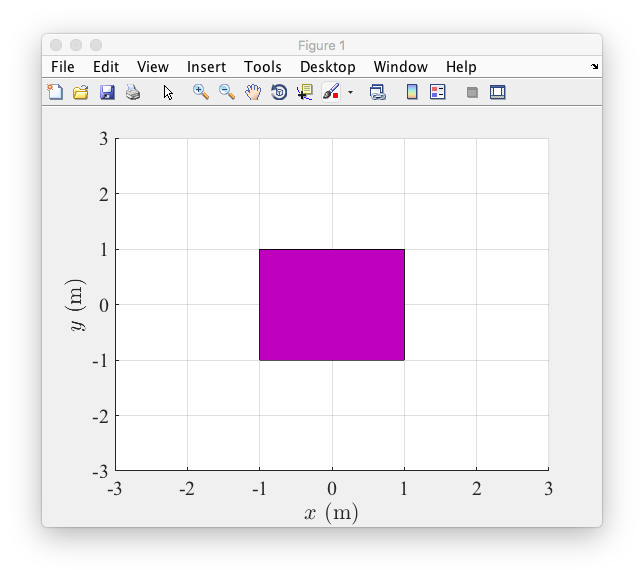
\includegraphics[width=0.475\textwidth]{graphics/basicPatchOutGraphical.png} \label{subfig:basicPatchOutputGraph}}
   \subfigure[ ]{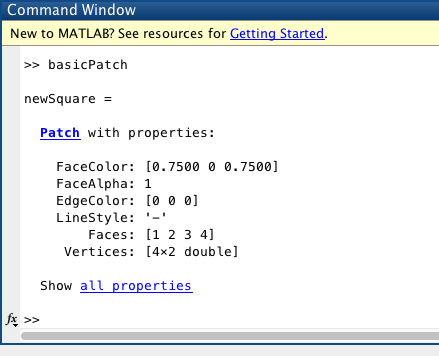
\includegraphics[width=0.475\textwidth]{graphics/basicPatchOutText.png} \label{subfig:basicPatchOutputText}}
   \caption{Graphical and Command Window output of the \texttt{basicPatch.m} script of Listing \ref{basicPatch}.}
   \label{fig:basicPatchOutput}
\end{figure}
% ^^^------------------------------------------------------------^^^

%The unsupressed output of Line 7 lists some properties of the \texttt{patch} object.
The \texttt{Patch} object is centered at the origin in Fig.\ \ref{subfig:basicPatchOutputGraph}. An example of a simple modification to this is to translate the patch by the vector $(\Delta x, \Delta y)$. To do this, we define $\Delta x$ and $\Delta y$, and add these to the original \texttt{XData} and \texttt{YData} properties of the \texttt{newSquare} object. This can be done in the Command Window using the \texttt{set()} function:
% vvv------------------------------------------------------------vvv
\begin{lstlisting}[style=Matlab-editor,label=basicPatchDisplace,caption={A Command Window modification to the \texttt{patch} defined in Listing \ref{basicPatch}. Line 1 is used to specify the $x$- and $y$-components of the displacement. The displacement is then applied to the original \texttt{XData} and \texttt{YData} properties, and the result of the addition is the value component of a property-value pair in the \texttt{set()} function.}]
>> Dx = -2; Dy = 1.5;
>> set(newSquare, 'XData', newSquare.XData + Dx, 'YData', newSquare.YData + DY)
\end{lstlisting}
% ^^^------------------------------------------------------------^^^
The syntax here is \verb!set(obj, Prop1, Val1, Prop2, Val2, ...)!, where \texttt{obj} is the object we wish to modify, and we use property-value pairs to assign new object properties. The displaced \texttt{patch} object is displayed in Fig.\ \ref{fig:basicPatchDisplaced}. Similar modifications may be made to a \texttt{line}-class object.

% vvv------------------------------------------------------------vvv
\begin{figure}[htbp] %  figure placement: here, top, bottom, or page
   \centering
   \subfigure[ \label{fig:basicPatchDisplaced}]{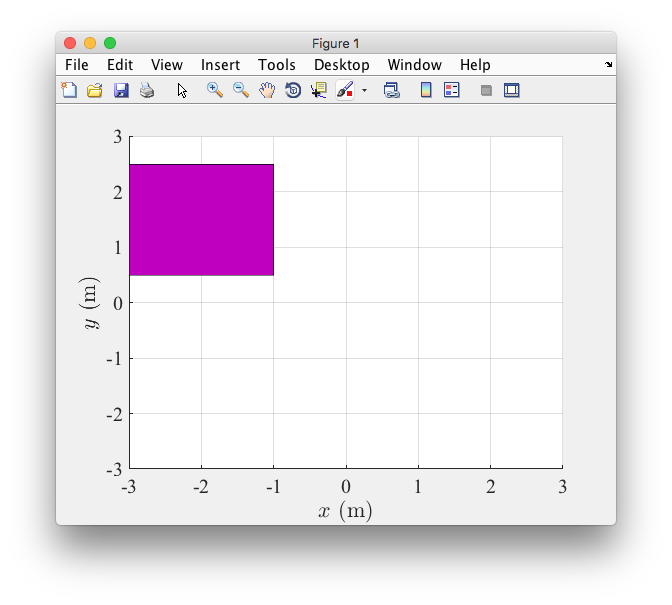
\includegraphics[width=0.475\textwidth]{graphics/basicPatchDisplaced.png}}
   \subfigure[ \label{fig:AxisEq}]{\includegraphics[width=0.475\textwidth]{graphics/FigPatchAxisEqual.png} \label{subfig:basicPatchOutputGraph}}
      \caption{(a) The \texttt{patch} object created using \texttt{basicPatch.m} is modified by using the \texttt{set()} function using the code of Listing \ref{basicPatchDisplace}. The resulting \texttt{patch} no longer sits at the origin. (b) The axes aspect ratio is made to be equal.}

\end{figure}
% ^^^------------------------------------------------------------^^^

You may have noticed that the aspect ratio is not equal for the plot of Figure \ref{fig:basicPatchDisplaced}. This may be improved using the \texttt{axis()} function:
% vvv------------------------------------------------------------vvv
\begin{lstlisting}[style=Matlab-editor,label=basicPatchDisplace,caption={A Command Window modification to the \texttt{patch} defined in Listing \ref{basicPatch}. Line 1 is used to specify the $x$- and $y$-components of the displacement. The displacement is then applied to the original \texttt{XData} and \texttt{YData} properties, and the result of the addition is the value component of a property-value pair in the \texttt{set()} function.}]
>> axis(gca, 'equal')
\end{lstlisting}
% ^^^------------------------------------------------------------^^^
This may adjust the \(x\)-limits and \(y\)-limits of the plot or only the positioning of the \texttt{Axis} object to get an equal aspect ratio.


For more information about the \texttt{patch} class, type \texttt{doc patch} in the MATLAB Command Window, or do an Internet search.


% ============================================================
\subsubsection{Animations using MATLAB Handle Graphics}
% ============================================================

When making animations in MATLAB, we may (1) replot each frame, or we may simply (2) adjust \texttt{XData}, \texttt{YData}, and \texttt{ZData} for objects in the plot for each frame. Method 2 is to be preferred, especially for interactive animations, because it is faster and avoids reconstructing and reformatting the plot. This results in a smoother experience for the user. It also may be helpful to set the axes limits using \texttt{xlim} and \texttt{ylim} so that relative positions of graphical objects is readily apparent between frames and the graphics for each frame all are plotted against the same background.

For an animation example and tutorial, see this demonstration on \myhref{https://youtu.be/mOwX0mfjJtQ}{animating ``rain drops''} in MATLAB.


% !TEX root = MATLAB_OOP_Blair.tex

% ============================================================
% ============================================================
% ============================================================
\section{Defining Classes in MATLAB}
% ============================================================
% ============================================================
% ============================================================

A class is a composite data type. MATLAB has several built-in classes, such as \texttt{figure}, and numerous graphics classes. MATLAB also allows you, the user, to define your own classes. To do so, you must write a class definition.

A class definition is a set of instructions defining for MATLAB your custom data type. A variables of a custom type is called an \textbf{object}.

\subsection{The Class-definition File}
In MATLAB, we define a class using a class-definition file. The file name must be identical to the name of the class itself, and it must have the '\texttt{.m}' extension. For example, to define an \texttt{Asset} class, we create a file named '\texttt{Asset.m}' (without the single quotes, of course).

A class definition file may be obtained by the `\texttt{New Document}' button on the \texttt{Home} tab of the MATLAB IDE and selecting the `\texttt{Class}' option. This opens a new editor window with a textual template for your new class. An example of a new class template is shown in Fig. \ref{fig:EditorNewClass}. Alternately, one can simply select a new script and write the class from scratch.

Let us examine some of the features of the template class file generated for us by MATLAB 2017b (see Fig. \ref{fig:EditorNewClass}):
\begin{enumerate}
\item The class definition files begins the keyword \texttt{classdef}, followed immediately by the class name (line 1). Also, lines of comments immediately follow line 1, providing help documentation for the class. Together, the documentation comments and line 1 provide a class header. 
\begin{itemize}
\item In this case, the class template has the text \texttt{untitled5} as a placeholder for the class name.
\end{itemize}

\item Following the class header, there are two sections to the class definition:
\begin{itemize}
\item The \textbf{properties section} begins with the key word \texttt{properties} (line 5) and ends with the key word \texttt{end} (line 7).

The body of the \texttt{properties} section is used to define class properties (also known as ``fields'', or ``member data''). Here, there is one dummy property defined: \texttt{Property1}.

\item The \textbf{methods section} begins with the key word \texttt{methods} (line 9) and ends with the key word \texttt{end} (line 21).

The body of the \texttt{methods} section is used to define functions which operate on objects. Such functions are more precisely called \textbf{methods}.

\begin{itemize}
\item The first method is an important function known as a \textbf{constructor} method. The constructor shares exactly the same name as the class, and is used to create or define an object of the class. A constructor typically receives input arguments which are used to specify some object properties. Typically, a constructor has a single output, \texttt{obj}, which is the desired result of the constructor. Of all the class methods, the constructor is unique in the sense that it does not operate on nor is it associated with an existing object. All other method functions operate on at least one object, and thus require an object as the first input argument, typically \texttt{obj}.

In particular, the placeholder constructor method \texttt{untitled5()} sums input arguments \texttt{inputArg1} and \texttt{inputArg2} and stores the result in the lone object property \texttt{Property1}.

\item The second method, \texttt{method1()}, is of the typical, non-constructor form. The first input argument is an object, \texttt{obj}. %We say that the class method \texttt{method1()} is associated with the object \texttt{obj}.
Within a non-constructor method, the object \texttt{obj} is only a copy of the object passed to the function in the first argument. In particular, \texttt{method1()} sums \texttt{inputArg} and the object property \texttt{obj.Property1} and returns this result as \texttt{outputArg}. This function does not modify the original object. In fact, within \texttt{method1()}, the code actually works with a copy of the object specified by \texttt{obj}.%modifies the \textit{temporary} copy of \texttt{obj} by adding the second argument \texttt{inputArg} to the \texttt{Property1} property.
% The output is typically an object, and often the same object \texttt{obj} as in the first input. Under such circumstances, the modified copy of \texttt{obj} is returned to the invoking script or function when the execution of \texttt{method1()} concludes. The modified copy of \texttt{obj} within \texttt{method1()} is then used to overwrite the original version of \texttt{obj} in the invoking testbed function, thus modifying the object.
\end{itemize}

\end{itemize}

\end{enumerate}

% vvv------------------------------------------------------------vvv
\begin{figure}[htbp] %  figure placement: here, top, bottom, or page
   \centering
   \subfigure[ ]{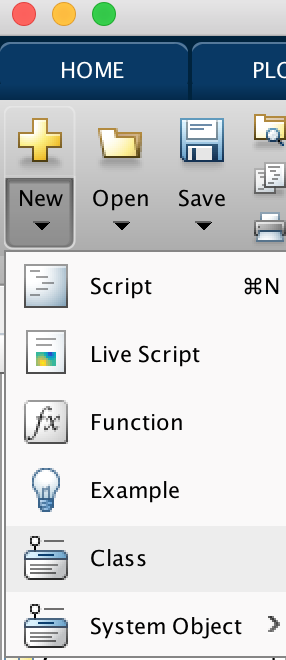
\includegraphics[height=2.5in]{graphics/NewDocumentClass.png}}
   \quad
   \subfigure[ ]{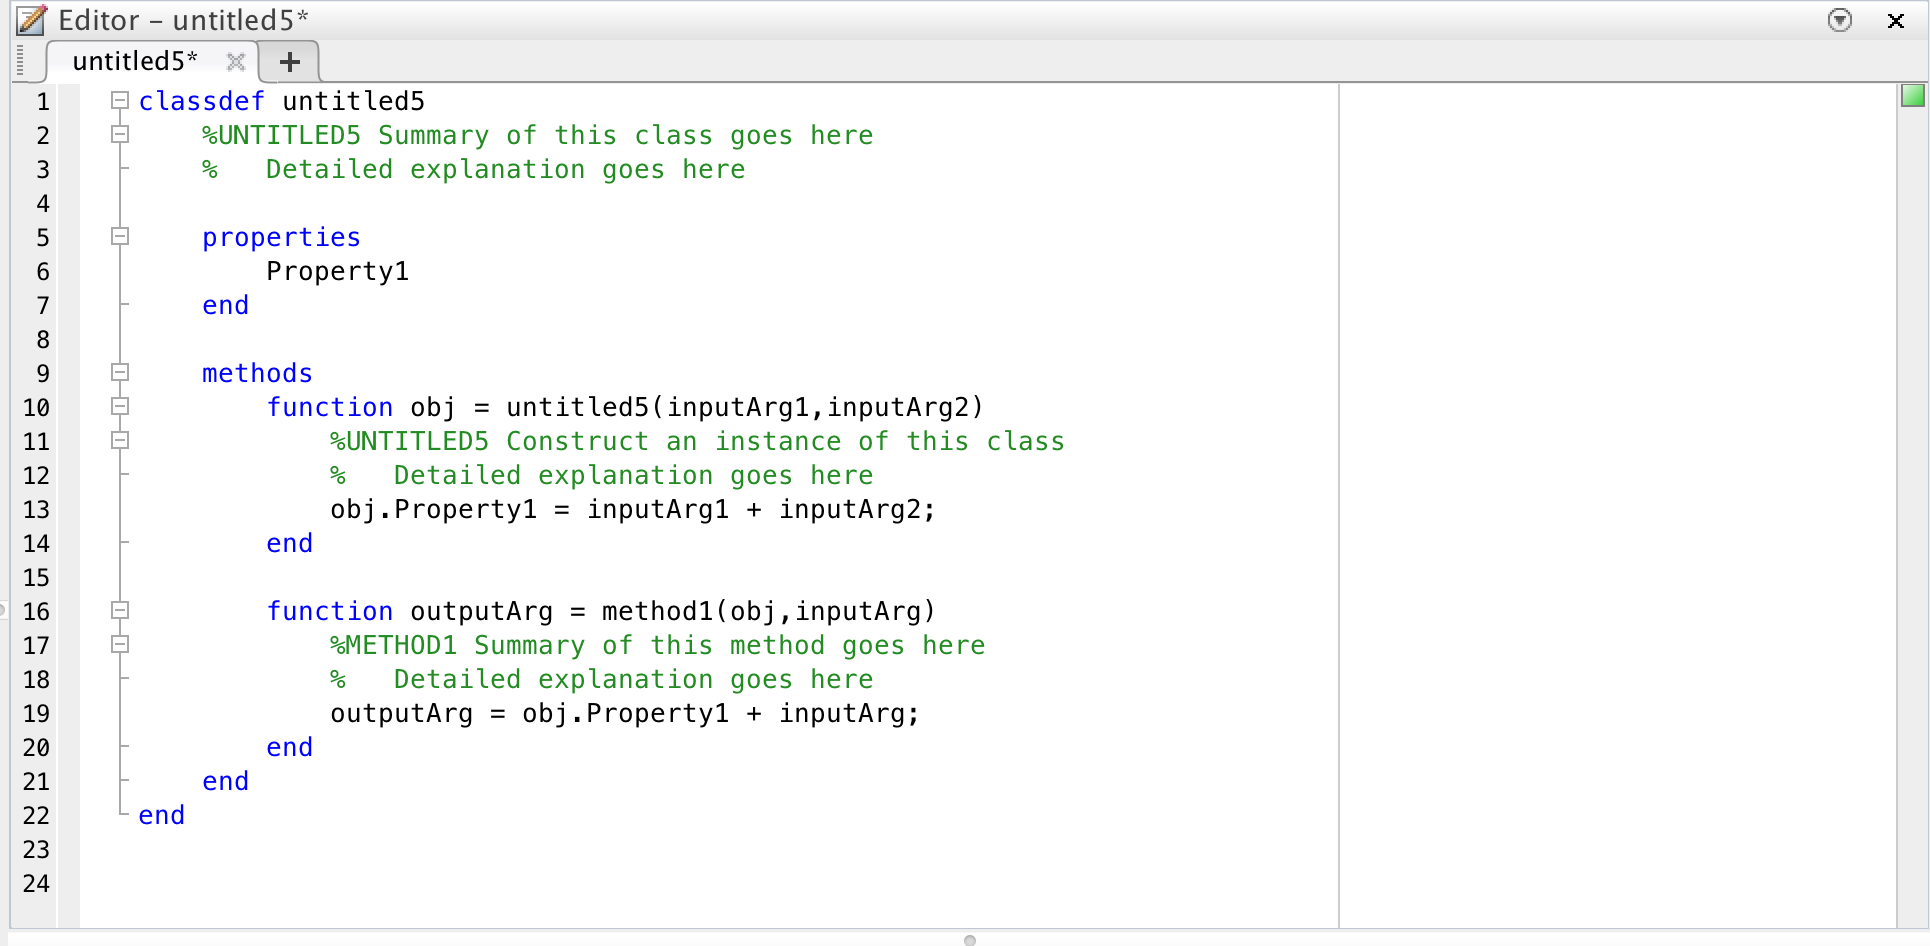
\includegraphics[height=2.5in]{graphics/MATLAB_Editor_NewClass.png}}
   \caption{(a) The ``New Document'' button provides a ``Class'' option. (b) A new class template obtained in MATLAB 2017b.}
   \label{fig:EditorNewClass}
\end{figure}
% ^^^------------------------------------------------------------^^^

\exmp{Example} \label{subsect:ConstructorUntitled5}
Create an object \texttt{myObj}.

\noindent \underline{Solution}.

To do this, we can invoke the constructor \texttt{untitled5()} using the syntax:
% vvv------------------------------------------------------------vvv
\begin{lstlisting}[style=Matlab-editor, caption={MATLAB Command Window input utilizing and testing the \texttt{untitled5} class definition of Fig.\ \ref{fig:EditorNewClass}.}]
>> x1 = 1; x2 = 2; myObj = untitled5(x1, x2)

myObj = 

  untitled5 with properties:

    Property1: 3
\end{lstlisting}
% ^^^------------------------------------------------------------^^^
Here, the command-line input of line 1 assigns the values 1 and 2 to \texttt{x1} and \texttt{x2}. Those values, then, are passed to the \texttt{untitled5()} constructor method to instantiate the object \texttt{myObj} of class \texttt{untitled5}. The output of this command is seen in lines 3-7, in which we see that \texttt{myObj} property \texttt{Property1} stores the value 3, which is the sum of the values stored in \texttt{x1} and \texttt{x2}.

\exmp{Invoke the method \texttt{method1()} on the object \texttt{myObj} created in Example \ref{subsect:ConstructorUntitled5}.}


\noindent \underline{Solution}.

To do this, invoke \texttt{method1()} using the syntax:
% vvv------------------------------------------------------------vvv
\begin{lstlisting}[style=Matlab-editor]
>> x = myObj.method1(5)

x =

     8
\end{lstlisting}
% ^^^------------------------------------------------------------^^^
To invoke \texttt{method1()} on \texttt{myObj}, we use the dot (``\texttt{.}'') syntax \texttt{myObj.method1(...)}, much like a reference to a property of \texttt{myObj}. This syntax is unique to class methods. While \texttt{myObj} does not appear within the input argument list to \texttt{method()} in line 1 above, it is in fact the first argument to \texttt{method()} because of the dot syntax. An alternative and equivalent\textemdash but older and depreciated\textemdash syntax for invoking \texttt{method1()} in line 1 above is \verb!x = method1(myObj, 5)!. This syntax explicitly specifies \texttt{myObj} as the first argument. The older syntax is used below, with the same result as above.
% vvv------------------------------------------------------------vvv
\begin{lstlisting}[style=Matlab-editor]
>> x = method1(myObj, 5)

x =

     8
\end{lstlisting}
% ^^^------------------------------------------------------------^^^

\subsubsection{Modifying Objects}
By default, when we pass an object to a method using either \texttt{obj.method1()} syntax or the older syntax, \textbf{only a copy of the object \texttt{obj} is passed to \texttt{method1()}}. Thus, any modifications \texttt{method1()} makes to its object are made to the \textit{copy}, not the original object.

If we wish to make a method \texttt{method2()} that modifies an object \texttt{myObj}, we need to define \texttt{method2()} in the following manner:
% vvv------------------------------------------------------------vvv
\begin{lstlisting}[style=Matlab-editor]
function obj = method2(obj, InputArg1, InputArg2, ... )
      < statements that modify obj >
end
\end{lstlisting}
% ^^^------------------------------------------------------------^^^
Now, \texttt{method2()} returns the modified copy of the input object. The syntax to modify \texttt{myObj} is as follows:
% vvv------------------------------------------------------------vvv
\begin{lstlisting}[style=Matlab-editor]
myObj = myObj.method2( a, b, ... );
\end{lstlisting}
% ^^^------------------------------------------------------------^^^
This invocation of \texttt{method2()} allows \texttt{method2()} to modify a copy of \texttt{myObj} inside the Workspace of \texttt{method2()}. Then, \texttt{method2()} returns a modified copy of \texttt{myObj}, which is used to overwrite the original, unmodified object \texttt{myObj}.


% ============================================================
% ============================================================
% ============================================================
\section{Extended Example: Developing Software to Track Investments}
% ============================================================
% ============================================================
% ============================================================

\subsection{Developing an \texttt{Asset} Class} \label{subsect:AssetClass}

Now we begin an extended, multi-part example, which begins with an \texttt{Asset} class. We will initially define an \texttt{Asset} class with the following properties: \texttt{name}, \texttt{symbol}, \texttt{quantity}, \texttt{units} and \texttt{transactionList}. Here \texttt{name} can store a \texttt{char} string to identify a company or mutual fund, and \texttt{symbol} can store a stock ticker symbol or equivalent symbol as a \texttt{char} string. The \texttt{units} property can store a \texttt{char} string specify the units of this asset: \texttt{'shares'}, \texttt{'USD'},  \texttt{'RMB'}, etc. Finally, the \texttt{transactionList} will store the list of transactions pertinent to the holdings in this asset. A transaction will be modeled as an object of the \texttt{Transaction} class, yet to be defined.

To do this, we prepare the class definition file \texttt{Asset.m}:
% vvv------------------------------------------------------------vvv
\begin{lstlisting}[style=Matlab-editor]
classdef Asset
    %Asset defines an Asset class to store information about a particular
    %investment asset (stock, mutual fund, currency, etc.).
    %
    % By E.P. Blair
    % Baylor University
    
    properties
        name
        symbol
        units
        transactionList
    end
    
    methods
        function obj = Asset(AName, ASymbol, AUnits)
            %Asset Constructs an instance (obj) of the Asset class
            %   Here, the required syntax is
            %   >> myObj = Asset( nameStr, symbolStr, unitStr )
            %   where nameStr, symbolStr, and unitsStr are char strings
            %   specifying the asset name, symbol, and units ('shares',
            %   'USD', 'RMB', etc.).
            obj.name = AName;
            obj.symbol = ASymbol;
            obj.units = AUnits;
        end
        
    end
end
\end{lstlisting}
% ^^^------------------------------------------------------------^^^
Here, in the \texttt{properties} section, lines 9-12 establish the desired class properties. The constructor of lines 16-26 is designed to accept three inputs: \texttt{AName}, \texttt{ASymbol}, and \texttt{AUnits}. The value of these parameters are then stored in the appropriate fields of the \texttt{Asset} object.

To test the \texttt{Asset} class definition, we can create a testbed script named \texttt{testbedAsset.m}:
% vvv------------------------------------------------------------vvv
\begin{lstlisting}[style=Matlab-editor]
% testbedAsset.m

newAsset = Asset('X-ray Yankee Zulu, Inc.', 'XYZ', 'shares')
\end{lstlisting}
% ^^^------------------------------------------------------------^^^
This script has one line, which simply invokes the \texttt{Asset} constructor to instantiate a new object, \texttt{newAsset}. The result of this testbed is:
% vvv------------------------------------------------------------vvv
\begin{lstlisting}[style=Matlab-editor]
>> testbedAsset

newAsset = 

  Asset with properties:

               name: 'X-ray Yankee Zulu, Inc.'
             symbol: 'XYZ'
              units: 'shares'
    transactionList: []
\end{lstlisting}
% ^^^------------------------------------------------------------^^^
Lines 2-10 list the output. Here, the required method inputs populate the appropriate object properties, and the \texttt{transactionList} remains empty.

% ========================================
\subsection{Developing a \texttt{Transaction} Class} \label{subsect:TransactionClass}
% ========================================

Now we will continue to develop the extended example started in Sect.\ \ref{subsect:AssetClass} by developing a \texttt{Transaction} class to have the following properties: \texttt{date}, \texttt{transactionType}, \texttt{quantity}, \texttt{price} and \texttt{fees}. Here, \texttt{date} can store an object of the pre-defined MATLAB class \texttt{datetime}; \texttt{transactionType} can store a \texttt{char} string to identify whether a transaction is a \texttt{'buy'}, \texttt{'sell'}, \texttt{'short'}, etc.; \texttt{quantity} and \texttt{price} can store a numerical value for the number of units transacted and the unit price, respectively; and, \texttt{fees} can be used to store transaction fees.

\noindent \underline{Solution}. 

% vvv------------------------------------------------------------vvv
\begin{lstlisting}[style=Matlab-editor]
classdef Transaction
    %Transaction defines a Transaction class to represent a transaction of
    %an investment assset, represented by the Asset class.
    %
    
    properties
        date % a MATLAB datetime object
        transactionType % 'buy', 'sell', 'short', 'dividend', 'split'
        quantity
        fee
        price
        
    end % END: properties
    
    methods
        function obj = Transaction( varargin )
            %Transaction constructs an instance of the Transaction class.
            %
            % SYNTAX:
            %
            % newTrans = Transaction( Ttype, Tquantity, Tprice)
            %     Defines a new transaction with the current date/time in
            %     the date field.
            %
            % newTrans = Transaction( Tdate, Ttype, Tquantity, Tprice)
            %     Defines a new transaction with a specified date/time. The
            %     date/time object may be specified as MATLAB datetime
            %     object or as a 3- or 6-element date vector.
            %
            % newTrans = Transaction( Tdate, Ttype, Tquantity, Tprice, fee)
            %     Defines a new transaction with a specified date/time and
            %     a transaction fee.
            %
            
            % This switch-case control group defines the Transaction object
            % differently based on the 
            switch nargin
                % The 3-input case assumes that the date is now
                case 3 % newTr = Transaction(Ttype, Tquantity, Tprice)
                    obj.date = datetime('now');
                    obj.transactionType = varargin{1};
                    obj.quantity = varargin{2};
                    obj.fee = 0;
                    obj.price = varargin{3};
                    
                % The 4-input case allows the transaction date to be
                % specified
                case 4 % newTr = Transaction(Tdate, Ttype, Tquantity, ...
                    %              Tprice)
                    
                    switch class(varargin{1})
                        case 'datetime'
                            obj.date = varargin{1};
                        case 'double' % the date specifier is in vector form
                            % convert a date vector to a datetime object
                            obj.date = datetime(varargin{1});
                        otherwise
                            error('Invalid transaction date specification.')
                    end
                    
                    obj.transactionType = varargin{2};
                    obj.quantity = varargin{3};
                    obj.price = varargin{4};
                    
                case 5
                    % newTr = Transaction( Tdate, Ttype, Tquantity, ...
                    %           Tprice, Tfee )
                    
                    switch class(varargin{1})
                        case 'datetime'
                            obj.date = varargin{1};
                        case 'double' % the date specifier is in vector form
                            % convert a date vector to a datetime object
                            obj.date = datetime(varargin{1});
                        otherwise
                            error('Invalid transaction date specification.')
                    end
                    
                    obj.transactionType = varargin{2};
                    obj.quantity = varargin{3};
                    obj.price = varargin{4};
                    obj.fee = varargin{5};
                    
                otherwise
                    error('Invalid number of input arguments.')
            end
            
        end
        

        
    end % END: methods
end
\end{lstlisting}
% ^^^------------------------------------------------------------^^^

The above listing defines the \texttt{Transaction} class, with only a constructor. In the \texttt{Transaction} constructor, fairly advanced techniques are used, such as a variable set of input arguments. Calls to the constructor are allowed with three, four, or five inputs. In the first (three-input) case, the \texttt{date} field is assumed to be the current date and time. The four-input and five-input cases allow the specification of the \texttt{date} property as either a date vector or as a \texttt{datetime} object (this is a pre-defined MATLAB class). To handle the different input cases, we use the \texttt{nargin} function along with a \texttt{switch}-\texttt{case} control sequence. A \texttt{switch}-\texttt{case} control also is used to enable the flexibility in the specification of the transaction date and time. See Appendix \ref{appendix:switch_case} for more information on \texttt{switch}-\texttt{case} controls.

We provide the testbed function \texttt{testbedTransaction.m} to test the class:
% vvv------------------------------------------------------------vvv
\begin{lstlisting}[style=Matlab-editor]
% testbedTransaction.m

% three-input constructor invocation
trans01 = Transaction( 'buy', 75, 71.90 )

% four-input constructor invocation with argument 1 as a date vector
trans02 = Transaction( [2017, 12, 1, 14, 30, 0], 'buy', 100, 7.19 )

% four-input constructor invocation with argument 1 as a datetime object
trans03 = Transaction( datetime('now'), 'sell', 25, 52 )

% five-input constructor to specify a transaction fee
trans04 = Transaction( datetime('now'), 'sell', 25, 52, 7 )
\end{lstlisting}
% ^^^------------------------------------------------------------^^^
The output of \texttt{testbedTransaction.m} demonstrates that the class definition works as designed:
% vvv------------------------------------------------------------vvv
\begin{lstlisting}[style=Matlab-editor]
>> testbedTransaction

trans01 = 

  Transaction with properties:

               date: 26-Dec-2017 11:13:15
    transactionType: 'buy'
           quantity: 75
                fee: 0
              price: 71.9000


trans02 = 

  Transaction with properties:

               date: 01-Dec-2017 14:30:00
    transactionType: 'buy'
           quantity: 100
                fee: []
              price: 7.1900


trans03 = 

  Transaction with properties:

               date: 26-Dec-2017 11:13:15
    transactionType: 'sell'
           quantity: 25
                fee: []
              price: 52


trans04 = 

  Transaction with properties:

               date: 26-Dec-2017 11:13:15
    transactionType: 'sell'
           quantity: 25
                fee: 7
              price: 52
\end{lstlisting}
% ^^^------------------------------------------------------------^^^

% ========================================
\subsection{Adding Transactions to an \texttt{Asset} Object} \label{subsect:AddTransaction}
% ========================================

Now we return to developing the \texttt{Asset} class. The goal here is to add transactions to an existing asset, say \texttt{someAsset}. We will treat the \texttt{transactionList} property as an array of type \texttt{Transaction}. If \texttt{transactionList} is empty, then the specified transaction is stored in the \texttt{transactionList} property. If the \texttt{transactionList} is not empty, then the new transaction should be added to the list, and transactions should be listed in chronological order.

\noindent \underline{Solution}.

We add an \texttt{addTransaction()} method to the \texttt{Asset} class definition file \texttt{Asset.m}. For clarity, we will use the notation \texttt{ClassName/methodName()} to remove any ambiguity regarding the class with which a method is associated. Also, a method \texttt{Asset/listTransactions()} which will compactly list the details of all transactions. This will help us test how well the \texttt{addTranstion()} method works. The updated class definition looks like this:
% vvv------------------------------------------------------------vvv
\begin{lstlisting}[style=Matlab-editor]
classdef Asset
    %Asset defines an Asset class to store information about a particular
    %investment asset (stock, mutual fund, currency, etc.).
    %
    % By E.P. Blair
    % Baylor University
    
    properties
        name = 'X-ray Yankee Zulu'
        symbol = 'XYZ'
        units = 'shares'
        transactionList
    end
    
    methods
        function obj = Asset(AName, ASymbol, AUnits)
            %Asset Constructs an instance (obj) of the Asset class
            %   Here, the required syntax is
            %   >> myObj = Asset( nameStr, symbolStr, unitStr )
            %   where nameStr, symbolStr, and unitsStr are char strings
            %   specifying the asset name, symbol, and units ('shares',
            %   'USD', 'RMB', etc.).
            obj.name = AName;
            obj.symbol = ASymbol;
            obj.units = AUnits;
        end
        
        function obj = addTransaction(obj, newTransaction)
            % addTransaction() adds a transaction newTransaction to the
            % transactionList property of obj
            
            % add the transaction on the end of the list
            obj.transactionList = [obj.transactionList newTransaction];
            
            % if the length of the list is greater than 1, the list may
            % require sorting
            
            if length(obj.transactionList) > 1
                % Create a list of transaction dates by iterating through
                % all transactions and adding dates to dateList
                dateList = []; % empty date list
                for TransIdx = 1:n_trans_old+1
                    % append the date of obj.transactionList(TransIdx) to
                    % dateList (unsorted)
                    dateList = [dateList ...
                        obj.transactionList(TransIdx).date];
                end
                
                % sort the transaction list
                
                % obtain an index of sorted transaction dates
                %   The sort function returns the sorted list along with
                %   the indices of sorted lists within the unsorted list
                %   The indices of the dateList, sortIndex, will be used to
                %   sort the list of transactions.
                [~, sortIndex] = sort(dateList);
                
                % reorder the unsorted transactions and store in
                % obj.transactionList
                obj.transactionList = obj.transactionList(sortIndex);
            end % END: if length(obj.transactionList) > 1
                
        end
        
        function obj = listTransactions(obj)
            numTrans = length(obj.transactionList);
            
            if numTrans > 0
                for transIndex = 1:numTrans
                    obj.transactionList(transIndex).listDetails;
                end
            else
                disp(['Asset ', obj.name, ' (', obj.symbol, ...
                    ') has no transactions.'])
            end
            
        end

        
    end % END: methods
end
\end{lstlisting}
% ^^^------------------------------------------------------------^^^
The new \texttt{Asset/addTransaction()} method is the first non-constructor method we've added to the \texttt{Asset} class. It works by first appending the new \texttt{Transaction} on the end of the \texttt{transactionList} property. If the total number of transactions \textemdash including the newly-appended transaction \textemdash is greater than 1, then the list may require sorting, so we will sort it regardless of whether it requires sorting (it may take even more work to figure out if the list requires sorting). Since the object \texttt{obj} is only a copy of the original \texttt{obj} upon which \texttt{addTransaction()} was invoked, we pass the modified copy \texttt{obj} out as an output argument.

The sorting uses the sort command. For a sortable array of elements \texttt{x}\textemdash such as \texttt{double}s or \texttt{datetime} objects, as in the present case\textemdash the \verb![x_sort, sortIndex] = sort(x)! returns a sorted version of \verb!x! in the output \verb!x_sort!, as well as the matching sequence of indices required to sort the original array \verb!x!. This sequence, \verb!sortIndex!, then is used to sort other pieces of data associated with the original array \texttt{x}. This is applied in \verb!addTransaction()! when we create \texttt{dateList}, an array of \texttt{datetime} objects associated with an array of \verb!Transaction! objects (line 45) and subsequently use the \texttt{sort()} command on \texttt{dateList}. We will not make direct use of a sorted list of dates, so we use \verb!~! to avoid storing that data in memory within the function \texttt{addTransaction}. However, the array \verb!sortIndex! will be used to sort the associated \verb!obj.transactionList! itself.

The \texttt{Asset/listTransactions()} method of lines 65-77 will be used to list the details of all \texttt{Transaction} objects associated with an \texttt{Asset} object. It is designed to use a \texttt{for} loop to iterate through all \texttt{Transaction} objects, and to print the details of each transaction using a \texttt{Transaction} method \texttt{listDetails()}, which remains to be defined.

This is an example of hierarchical programming: a user can instruct an \texttt{Asset} object to list its transaction details by invoking the \texttt{Asset/listTransactions()} method. \texttt{Asset/listTransactions()} method, in turn, invokes the \texttt{Transaction/listDetails()} method for each associated \texttt{Transaction} object. We list below \texttt{Transaction} class definition, upgraded with a definition for the \texttt{listDetails()} method:
% vvv------------------------------------------------------------vvv
\begin{lstlisting}[style=Matlab-editor]
classdef Transaction
    %Transaction defines a Transaction class to represent a transaction of
    %an investment assset, represented by the Asset class.
    %
    
    properties
        date % a MATLAB datetime object
        transactionType % 'buy', 'sell', 'short', 'dividend', 'split'
        quantity
        fee
        price
        
    end % END: properties
    
    methods
        function obj = Transaction( varargin )
            %Transaction constructs an instance of the Transaction class.
            %
            % SYNTAX:
            %
            % newTrans = Transaction( Ttype, Tquantity, Tprice)
            %     Defines a new transaction with the current date/time in
            %     the date field.
            %
            % newTrans = Transaction( Tdate, Ttype, Tquantity, Tprice)
            %     Defines a new transaction with a specified date/time. The
            %     date/time object may be specified as MATLAB datetime
            %     object or as a 3- or 6-element date vector.
            %
            % newTrans = Transaction( Tdate, Ttype, Tquantity, Tprice, fee)
            %     Defines a new transaction with a specified date/time and
            %     a transaction fee.
            %
            
            % This switch-case control group defines the Transaction object
            % differently based on the 
            switch nargin
                % The 3-input case assumes that the date is now
                case 3 % newTr = Transaction(Ttype, Tquantity, Tprice)
                    obj.date = datetime('now');
                    obj.transactionType = varargin{1};
                    obj.quantity = varargin{2};
                    obj.fee = 0;
                    obj.price = varargin{3};
                    
                % The 4-input case allows the transaction date to be
                % specified
                case 4 % newTr = Transaction(Tdate, Ttype, Tquantity, ...
                    %              Tprice)
                    
                    switch class(varargin{1})
                        case 'datetime'
                            obj.date = varargin{1};
                        case 'double' % the date specifier is in vector form
                            % convert a date vector to a datetime object
                            obj.date = datetime(varargin{1});
                        otherwise
                            error('Invalid transaction date specification.')
                    end
                    
                    obj.transactionType = varargin{2};
                    obj.quantity = varargin{3};
                    obj.price = varargin{4};
                    
                case 5
                    % newTr = Transaction( Tdate, Ttype, Tquantity, ...
                    %           Tprice, Tfee )
                    
                    switch class(varargin{1})
                        case 'datetime'
                            obj.date = varargin{1};
                        case 'double' % the date specifier is in vector form
                            % convert a date vector to a datetime object
                            obj.date = datetime(varargin{1});
                        otherwise
                            error('Invalid transaction date specification.')
                    end
                    
                    obj.transactionType = varargin{2};
                    obj.quantity = varargin{3};
                    obj.price = varargin{4};
                    obj.fee = varargin{5};
                    
                otherwise
                    error('Invalid number of input arguments.')
            end
            
        end
        
        
        function listDetails(obj)
            DateString = [char(obj.date) ...
                blanks(20 - length(char(obj.date)) ) ];
            TypeString = [blanks(10-length(obj.transactionType)), ...
                obj.transactionType];
            
            QtyString = [blanks(10 - length(num2str(obj.quantity))), ...
                num2str(obj.quantity)];
            
            RawPriceStr = num2str(obj.price, '%0.3g');
            PriceString = [' at ', blanks(10 - length(RawPriceStr)), ...
                RawPriceStr];
            
            DetailString = [DateString, TypeString, QtyString, PriceString];
            
            disp(DetailString)
        end
        
    end % END: methods
end
\end{lstlisting}
% ^^^------------------------------------------------------------^^^

Additionally, we add some functionality to the \texttt{Transaction} class. We add a method \texttt{listDetails} that lists the details of a \texttt{Transaction} object. The upgraded \texttt{Transaction} class is listed in 91-107. Here, we define several strings of fixed width. First, we use the \texttt{char} method defined for \texttt{datetime} objects to generate a \texttt{char} string representing the transaction date (see line 91-92). This string has length \verb!length(char(obj.date))!. We use the \texttt{blanks()} function to right-pad this string with white space so that \texttt{DateString} is a length of 20 characters always.  In line 93, we include the string contained in the \texttt{obj.transactionType} property as part of the string \texttt{TypeString} but we use the \texttt{blanks()} function to left-pad the \texttt{obj.transactionType} string with white spaces. This forms \texttt{TypeString} as a 10-character string. We use the same technique in line 97 to create a 10-character string detailing the number of units transacted stored in the \texttt{obj.quantity} property. Here, the \texttt{num2str()} function is used to convert the \texttt{double} data representing the number of units transacted to a \texttt{char} string. Similarly, lines 100-101 form a fixed-length \texttt{char} string \texttt{PriceString} detailing the price per unit of the transaction. Finally, in line 104, \texttt{DateString}, \texttt{TypeString}, \texttt{QtyString}, and \texttt{PriceString} are concatenated in one string \texttt{DetailString}. Then, in line 106, the \texttt{disp()} function is used to print \texttt{DetailString} to the Command Window output. All of this functionality is called simply within the \texttt{Asset} \texttt{listTransactions} method by invoking the \texttt{Transaction} class \texttt{listDetails} method for each \texttt{Transaction} object.

A modified version of \texttt{testbedAsset.m} is shown here, in Listing \ref{lst:testbedAsset02}:
% vvv------------------------------------------------------------vvv
\begin{lstlisting}[style=Matlab-editor, caption={The code listing for \texttt{testbedAsset.m}. Here, the testbed adds transactions to \texttt{newAsset} and invokes the \texttt{listTransactions} method to display information about associated \texttt{Transaction} objects.}, label={lst:testbedAsset02}]
% testbedAsset.m

% create an new Asset object with no transactions
newAsset = Asset('X-ray Yankee Zulu, Inc.', 'XYZ', 'shares')

% add a buy transaction with the current date
newAsset = newAsset.addTransaction( Transaction('buy', 100, 24.03) )

% list transaction data after the first addition
newAsset.listTransactions;

% add a transaction with an earlier date
newAsset = newAsset.addTransaction( Transaction([2017, 12, 1], ...
    'buy', 25, 22.97) )

% list transaction data after the first addition
newAsset.listTransactions;
\end{lstlisting}
% ^^^------------------------------------------------------------^^^
The output of \texttt{testbedAsset.m} is shown below:
% vvv------------------------------------------------------------vvv
\begin{lstlisting}[style=Matlab-editor, caption={The output of \texttt{testbedAsset.m}}, label={lst:AssetOutput02}]
>> testbedAsset

newAsset = 

  Asset with properties:

               name: 'X-ray Yankee Zulu, Inc.'
             symbol: 'XYZ'
              units: 'shares'
    transactionList: []


newAsset = 

  Asset with properties:

               name: 'X-ray Yankee Zulu, Inc.'
             symbol: 'XYZ'
              units: 'shares'
    transactionList: [1x1 Transaction]

Transactions for X-ray Yankee Zulu, Inc. (XYZ):
26-Dec-2017 21:36:04       buy       100 at         24

newAsset = 

  Asset with properties:

               name: 'X-ray Yankee Zulu, Inc.'
             symbol: 'XYZ'
              units: 'shares'
    transactionList: [1x2 Transaction]

Transactions for X-ray Yankee Zulu, Inc. (XYZ):
01-Dec-2017                buy        25 at         23
26-Dec-2017 21:36:04       buy       100 at         24
\end{lstlisting}
% ^^^------------------------------------------------------------^^^
Line 3 of Listing \ref{lst:testbedAsset02} resulted in output lines 3-10. Here, we see that \texttt{newAsset} has an empty \texttt{transactionList} array property. Line 7 of Listing \ref{lst:testbedAsset02} adds a new transaction, resulting in output lines 13-20 here. This shows that \texttt{newAsset} now has one transaction. Line 10 of Listing \ref{lst:testbedAsset02} invokes the \texttt{listTransactions()} method for \texttt{newAsset}, resulting in output lines 22-23 here. Next, a second, earlier, transaction is added in line 13 of Listing \ref{lst:testbedAsset02}. This results in the output of lines 25-32 here. When we again invoke the \texttt{listTransactions()} method, we see that not only does \texttt{newAsset} have two transactions, but the transactions are listed in chronological order from earliest to latest.

% ========================================
\subsection{Calculating the Value of Holdings in an \texttt{Asset}} \label{subsect:CalculateAssetValue}
% ========================================

To calculate the value of holdings in an asset, we will add a method \texttt{Asset/calculateValue()}. This will iterate through all the \texttt{Transaction} objects stored in an \texttt{Asset} object's \texttt{transactionList}. For each transaction, \texttt{Asset/calculateValue()} determine how that transaction will affect the holdings and determine the cost of that transaction based on the type of the transaction and the number of units transacted. In support of this, we first list some upgrades and changes to the \texttt{Transaction} class. Changes and upgrades are as follows:
\begin{itemize}
\item To support dividend and split transactions, the following class properties are added: \texttt{dividend}, \texttt{split\_ratio})
\item Some properties (\texttt{quantity}, \texttt{dividend}, \texttt{split\_ratio}) are assigned a default value. This is done by using an assignment operator and the desired default value along with the property declaration in the \texttt{properties} section (syntax: \texttt{Property = defaultValue;}).
\item The \texttt{Transaction} constructor four-input case (inside the \texttt{switch nargin} control block) is augmented with a \texttt{switch obj.transactionType}-\texttt{case} to handle \texttt{div-rnv} (dividend reinvestment) transactions. Here, in the \texttt{'div-rnv'} case, the third argument is not the quantity of units transacted, but rather a total dollar amount. The fourth argument remains the price per unit, and this enables the calculation of units bought with a reinvested dividend.
\end{itemize}
The upgraded \texttt{Transaction} class definition is listed below.
% vvv------------------------------------------------------------vvv
\begin{lstlisting}[style=Matlab-editor, caption={The \texttt{Transaction} class, as enhanced to support \texttt{Asset} value calculations.}, label={lst:TransactionForCalculations}]
classdef Transaction
    %Transaction defines a Transaction class to represent a transaction of
    %an investment assset, represented by the Asset class.
    %
    
    properties
        date % a MATLAB datetime object
        transactionType % 'buy', 'sell', 'short', 'dividend', 'split'
        quantity = 0;
        dividend = 0;
        split_ratio = 1;
        fee = 0; % Default value: zero
        price
        
    end % END: properties
    
    methods
        function obj = Transaction( varargin )
            %Transaction constructs an instance of the Transaction class.
            %
            % SYNTAX:
            %
            % newTrans = Transaction( Ttype, Tquantity, Tprice)
            %     Defines a new transaction with the current date/time in
            %     the date field. Valid transaction types are 'buy',
            %     'sell', and 'div-rnv' (dividend reinvestment).
            %
            % newTrans = Transaction( Tdate, Ttype, Tquantity, Tprice)
            %     Defines a new transaction with a specified date/time. The
            %     date/time object may be specified as MATLAB datetime
            %     object or as a 3- or 6-element date vector.
            %
            % newTrans = Transaction( Tdate, Ttype, Tquantity, Tprice, fee)
            %     Defines a new transaction with a specified date/time and
            %     a transaction fee.
            %
            
            % This switch-case control group defines the Transaction object
            % differently based on the 
            switch nargin
                % The 3-input case assumes that the date is now
                case 3 % newTr = Transaction(Ttype, Tquantity, Tprice)
                    obj.date = datetime('now');
                    obj.transactionType = varargin{1};
                    obj.quantity = varargin{2};
                    obj.fee = 0;
                    obj.price = varargin{3};
                    
                % The 4-input case allows the transaction date to be
                % specified
                case 4 % newTr = Transaction(Tdate, Ttype, Tquantity, ...
                    %              Tprice)
                    
                    switch class(varargin{1})
                        case 'datetime'
                            obj.date = varargin{1};
                        case 'double' % the date specifier is in vector form
                            % convert a date vector to a datetime object
                            obj.date = datetime(varargin{1});
                        otherwise
                            error('Invalid transaction date specification.')
                    end
                    
                    obj.transactionType = varargin{2};
                    
                    obj.price = varargin{4};
                    
                    switch obj.transactionType
                        case 'div-rnv'
                            obj.dividend = varargin{3};
                            obj.quantity = obj.dividend/obj.price;
                        otherwise
                            obj.quantity = varargin{3};
                    end
                    
                    
                case 5
                    % newTr = Transaction( Tdate, Ttype, Tquantity, ...
                    %           Tprice, Tfee )
                    
                    switch class(varargin{1})
                        case 'datetime'
                            obj.date = varargin{1};
                        case 'double' % the date specifier is in vector form
                            % convert a date vector to a datetime object
                            obj.date = datetime(varargin{1});
                        otherwise
                            error('Invalid transaction date specification.')
                    end
                    
                    obj.transactionType = varargin{2};
                    obj.quantity = varargin{3};
                    obj.price = varargin{4};
                    obj.fee = varargin{5};
                    
                otherwise
                    error('Invalid number of input arguments.')
            end
            
        end
        
        
        function listDetails(obj)
            DateString = [char(obj.date) ...
                blanks(20 - length(char(obj.date)) ) ];
            TypeString = [blanks(10-length(obj.transactionType)), ...
                obj.transactionType];
            
            QtyString = [blanks(10 - length(num2str(obj.quantity))), ...
                num2str(obj.quantity)];
            
            RawPriceStr = num2str(obj.price, '%0.3g');
            PriceString = [' at ', blanks(10 - length(RawPriceStr)), ...
                RawPriceStr];
            
            DetailString = [DateString, TypeString, QtyString, PriceString];
            
            disp(DetailString)
        end
        
    end % END: methods
end
\end{lstlisting}
% ^^^------------------------------------------------------------^^^

Next, we list the upgraded \texttt{Asset} class definition with the new \texttt{calculateValue()} function:
% vvv------------------------------------------------------------vvv
\begin{lstlisting}[style=Matlab-editor, caption={The \texttt{Asset} class with a new \texttt{calculateValue()} method.}, label={lst:AssetValueCalculation}]
classdef Asset
    %Asset defines an Asset class to store information about a particular
    %investment asset (stock, mutual fund, currency, etc.).
    %
    % By E.P. Blair
    % Baylor University
    
    properties
        name = 'X-ray Yankee Zulu'
        symbol = 'XYZ'
        units = 'shares'
        transactionList
    end
    
    methods
        function obj = Asset(AName, ASymbol, AUnits)
            %Asset Constructs an instance (obj) of the Asset class
            %   Here, the required syntax is
            %   >> myObj = Asset( nameStr, symbolStr, unitStr )
            %   where nameStr, symbolStr, and unitsStr are char strings
            %   specifying the asset name, symbol, and units ('shares',
            %   'USD', 'RMB', etc.).
            obj.name = AName;
            obj.symbol = ASymbol;
            obj.units = AUnits;
        end
        
        function obj = addTransaction(obj, newTransaction)
            % addTransaction() adds a transaction newTransaction to the
            % transactionList property of obj
            
            % add the transaction on the end of the list
            obj.transactionList = [obj.transactionList newTransaction];
            
            % if the length of the list is greater than 1, the list may
            % require sorting
            
            if length(obj.transactionList) > 1
                % Create a list of transaction dates by iterating through
                % all transactions and adding dates to dateList
                dateList = []; % empty date list
                for TransIdx = 1:length(obj.transactionList)
                    % append the date of obj.transactionList(TransIdx) to
                    % dateList (unsorted)
                    dateList = [dateList ...
                        obj.transactionList(TransIdx).date];
                end
                
                % sort the transaction list
                
                % obtain an index of sorted transaction dates
                %   The sort function returns the sorted list along with
                %   the indices of sorted lists within the unsorted list
                %   The indices of the dateList, sortIndex, will be used to
                %   sort the list of transactions.
                [~, sortIndex] = sort(dateList);
                
                % reorder the unsorted transactions and store in
                % obj.transactionList
                obj.transactionList = obj.transactionList(sortIndex);
            end % END: if length(obj.transactionList) > 1
                
        end
        
        function obj = listTransactions(obj)
            numTrans = length(obj.transactionList);
            
            if numTrans > 0
                disp(['Transactions for ', obj.name, ' (', obj.symbol, ...
                    '):'])
                for transIndex = 1:numTrans
                    obj.transactionList(transIndex).listDetails;
                end
                
            else
                disp(['Asset ', obj.name, ' (', obj.symbol, ...
                    ') has no transactions.'])
            end
            
        end

        function varargout = calculateValue(obj)
            % Asset/calculateValue performs an analysis on the list of
            % transactions to calculate asset holdings and their value at
            % the time of the last transaction.
            % 
            % Syntax:
            %
            % Value = myAsset.calculateValue returns the value of holdings
            %     at the time of the last transaction.
            %
            % [Value, Units] = myAsset.calculateValue additionally returns
            %     the total number of units held.
            %
            % [Value, Units, CostBasis] = myAsset.calculateValue returns
            %     the investor's cost basis.
            %
            
            Value = 0; % value of holdings
            TotalUnits = 0; % number of units held
            CostBasis = 0; % cost basis of investment
            if ~isempty(obj.transactionList)
                numTrans = length(obj.transactionList);
                
                % Units: storage vector for units owned as a fcn. of time
                Units = zeros(1, numTrans);
                Cost = zeros(1, numTrans);
                Value = zeros(1, numTrans);
                
                % Iterate through all transitions
                for transIdx = 1:numTrans
                    % extract a single transition
                    tempTrans = obj.transactionList(transIdx);
                    
                    if transIdx == 1
                        Units(1) = tempTrans.quantity;
                        Cost(transIdx) = tempTrans.price ...
                            * tempTrans.quantity ...
                            + tempTrans.fee;
                        
                    else
                        
                        
                        switch tempTrans.transactionType
                            case 'buy'
                                Units(transIdx) = Units(transIdx-1) ...
                                    + tempTrans.quantity;

                                Cost(transIdx) = tempTrans.price ...
                                    * tempTrans.quantity ...
                                    + tempTrans.fee;
                                
                            case 'sell'
                                Units(transIdx) = Units(transIdx-1) ...
                                    - tempTrans.quantity;
                                Cost(transIdx) = -tempTrans.price ...
                                    * tempTrans.quantity ...
                                    + tempTrans.fee;
                                
                            case 'split'
                                Units(transIdx) = Units(transIdx-1) ...
                                    * tempTrans.split_ratio;
                                
                            case 'div-rnv'
                                Units(transIdx) = Units(transIdx-1) ...
                                    + tempTrans.dividend/tempTrans.price;
                                
                        end
                        
                        
                    end

                end % END: for transIdx = 1:numTrans 
                
                CostBasis = sum(Cost);
                Qty = Units(end);
                Value = Qty*tempTrans.price; %
                LastPrice = tempTrans.price;
                
            end
            
            
            switch nargout
                case 1
                    varargout{1} = Value;
                case 2
                    varargout{1} = Value;
                    varargout{2} = Qty;
                case 3
                    varargout{1} = Value;
                    varargout{2} = Qty;
                    varargout{3} = CostBasis;
                case 4
                    varargout{1} = Value;
                    varargout{2} = Qty;
                    varargout{3} = CostBasis;
                    varargout{4} = LastPrice;

                otherwise
                    error('Invalid number of output arguments.')
            end
            
        end
        
    end % END: methods
end
\end{lstlisting}
% ^^^------------------------------------------------------------^^^

The new \texttt{Asset/calculateValue()} method is listed in lines 82-174 of Listing \ref{lst:AssetValueCalculation}.  The function header uses \texttt{varargout} (a variable-length set of output arguments) to allow the user flexibility in outputs. The help documentation comments provide information about the syntax; and a \texttt{switch}-\texttt{case} control (lines 160-172) manages the outputs depending on \texttt{nargout}, the number of outputs  in the particular function invocation.

Finally, we list a new testbed script, \texttt{testbedAssetv02.m} (see Listing \ref{lst:AssetValueCalculationTestbed}). This defines an \texttt{Asset} object \texttt{newAsset}. It adds several transactions to \texttt{newAsset} and lists them using the \texttt{Asset} method \texttt{listTransactions()}. Finally, the script invokes the \texttt{Asset/calculateValue()} method and lists data calculated for this asset. Here, one \texttt{disp()} command was used, and the command \texttt{char(10)} embeds character ten (the MATLAB code for a newline character) in the string and breaks the string up for readability.
% vvv------------------------------------------------------------vvv
\begin{lstlisting}[style=Matlab-editor, caption={A testbed function for \texttt{Asset} value calculations.}, label={lst:AssetValueCalculationTestbed}]
% testbedAssetv02.m

% create an new Asset object with no transactions
newAsset = Asset('X-ray Yankee Zulu, Inc.', 'XYZ', 'shares');

% add a buy transaction with the current date
newAsset = newAsset.addTransaction( Transaction('sell', 40, 24.03) );

% list transaction data after the first addition
newAsset.listTransactions;

% add a transaction with an earlier date
newAsset = newAsset.addTransaction( Transaction([2017, 1, 1], ...
    'buy', 25, 22.97) );

% add a transaction with an earlier date
newAsset = newAsset.addTransaction( Transaction([2017, 3, 18], ...
    'div-rnv', 40, 23.58) );

% add a transaction with an earlier date
newAsset = newAsset.addTransaction( Transaction([2017, 5, 24], ...
    'buy', 100, 25.17) );

% list transaction data after the first addition
newAsset.listTransactions;

[Value, Holdings, CostBasis] = newAsset.calculateValue;
Gain = Value - CostBasis;

disp([char(10), 'Asset           : ', newAsset.name, ' (', newAsset.symbol, ...
    ')', char(10), 'Quantity        : ', num2str(Holdings), ...
    char(10), 'Value           : $', num2str(Value), ...
    char(10), 'Cost Basis      : $', num2str(CostBasis), ...
    char(10), 'Unrealized Gains: $', num2str(Gain), ...
    ' or ', num2str(100*Gain/CostBasis, '%0.4g'), '%'])
\end{lstlisting}
% ^^^------------------------------------------------------------^^^
Running the testbed script of Listing \ref{lst:AssetValueCalculationTestbed} yields the output of Listing \ref{lst:AssetValueCalculationTestbedOutput}.
% vvv------------------------------------------------------------vvv
\begin{lstlisting}[style=Matlab-editor, caption={Output for the testbed function of Listing \ref{lst:AssetValueCalculationTestbed}.}, label={lst:AssetValueCalculationTestbedOutput}]
>> testbedAssetv02
Transactions for X-ray Yankee Zulu, Inc. (XYZ):
29-Dec-2017 20:46:36      sell        40 at         24
Transactions for X-ray Yankee Zulu, Inc. (XYZ):
01-Jan-2017                buy        25 at         23
18-Mar-2017            div-rnv    1.6964 at       23.6
24-May-2017                buy       100 at       25.2
29-Dec-2017 20:46:36      sell        40 at         24

Asset           : X-ray Yankee Zulu, Inc. (XYZ)
Quantity        : 86.6964
Value           : $2083.3134
Cost Basis      : $2130.05
Unrealized Gains: $-46.7366 or -2.194%
\end{lstlisting}
% ^^^------------------------------------------------------------^^^
Some additional formatting may be desired for dollar and percentage amounts.

% ============================================================
% ============================================================
% ============================================================
\subsection{A \texttt{Portfolio} Class: a Container Class for \texttt{Asset} Objects}
% ============================================================
% ============================================================
% ============================================================

Here, we will define a \texttt{Portfolio} class that serves as a container class for \texttt{Asset} objects. Actually, we already created the \texttt{Asset} class as a container for \texttt{Transaction} objects. The \texttt{Portfolio} class will be built with an \texttt{addAsset()} method and a \texttt{calculateValue()} method. The \texttt{Portfolio} \texttt{calculateValue()} method will hierarchically calculate its own value by invoking the \texttt{Asset} class \texttt{calculateValue()} method for each \texttt{Asset} object held in the portfolio.

% vvv------------------------------------------------------------vvv
\begin{lstlisting}[style=Matlab-editor, caption={The class definition for \texttt{Portfolio}, a container class for objects of class \texttt{Asset}.}, label={lst:PortfolioClass}]
classdef Portfolio
    %PORTFOLIO defines a container class Portfolio for objects of type
    %   Asset. A Portfolio object calculates its own value by calling each
    %   contained Asset object to evaluate and return its individual value.
    %
    
    properties
        name
        assetList
    end
    
    methods
        function obj = Portfolio(varargin)
            %Portfolio constructs an Portfolio object.
            %
            %   SYNTAX:
            %
            %   myPortfolio = Portfolio creates an empty portfolio.
            %
            %   myPortfolio = Portfolio( portfolioName, assetArray )
            %   Detailed explanation goes here
            
            switch nargin
                case 0
                    obj.name = 'Default Portfolio';
                    obj.assetList = [];
                    
                case 2
                    obj.name = varargin{1};
                    if strcmp(class(varargin{2}), 'Asset') % input checking
                        obj.assetList = varargin{2};
                    else
                        error('Non-Asset object specified for asset list.')
                    end

            end 
        end % END: Portfolio constructor
        
        function obj = addAssets(obj, additionalAssets)
            % Portfolio/addAsset adds new Asset objects to the assetList
            %   property of a Portfolio object.
            %
            % SYNTAX:
            %
            % myPortfolio = myPortfolio.addAsset( additionalAssets )
            %   
            if strcmp(class(additionalAssets), 'Asset') % input checking
                obj.assetList = [obj.assetList additionalAssets];
            else
                error('Non-Asset object specified for asset list.')
            end    
        end % END: Portfolio/addAssets()
        
        function varargout = calculateValue(obj)
            
            PortfolioValue = 0;
            PortfolioData = [];
            
            if ~isempty(obj.assetList)
                numAssets = length(obj.assetList);
                Symbol = cell(numAssets, 1);
                Value = zeros(numAssets, 1); % storage vector
                Holdings = Value; % storage vector
                CostBasis = Value; % storage vector
                UnitPrice = Value;
                for AssetIdx = 1:numAssets
                    tempAsset = obj.assetList(AssetIdx);
                    [Value(AssetIdx), Holdings(AssetIdx), ...
                        CostBasis(AssetIdx), ...
                        UnitPrice(AssetIdx)] = tempAsset.calculateValue;
                    Symbol{AssetIdx} = tempAsset.symbol;
                end
                UnrealizedGains = Value - CostBasis;
                
                PortfolioValue = sum(Value);
                PortfolioData = table(Symbol, Value, Holdings, ...
                    UnitPrice, CostBasis, UnrealizedGains);
            end
                
            switch nargout 
                case 1
                    varargout{1} = PortfolioValue;
                case 2
                    varargout{1} = PortfolioValue;
                    varargout{2} = PortfolioData;
                otherwise
                    error('Invalid number of outputs specified.')
            end
                    
        end % END: Portfolio/calculateValue()
    end
end
\end{lstlisting}
% ^^^------------------------------------------------------------^^^

The key property of \texttt{Portfolio} in Listing \ref{lst:PortfolioClass} is the \texttt{assetList} property. This property will store a horizontal concatenation of \texttt{Asset} objects. The concatenation is seen in the \texttt{Portfolio} class \texttt{addAssets()} method. Finally, the \texttt{Portfolio} class \texttt{calculateValue()} method invokes the \texttt{Asset} class \texttt{calculateValue()} method on \texttt{Asset} objects contained by the \texttt{Portfolio} object. For each \texttt{Asset} object, \texttt{Portfolio} \texttt{calculateValue()} method saves information about holdings at the last transaction, including: value, total holdings, unit price, symbol, and the price per unit.  This data then is combined in a MATLAB \texttt{table} object. 

Next, I list a testbed function, \texttt{testbedPortfolio.m} in Listing \ref{lst:PortfolioTestbed}. Here, two \texttt{Asset} objects are created, and several \texttt{Transaction} objects are added to each. Then, the two \texttt{Asset} objects are added to a new \texttt{Portfolio} object using the \texttt{Portfolio} method \texttt{addAssets()}. Finally, the \texttt{Portfolio} method \texttt{calculateValue()} is invoked on the new \texttt{Portfolio} object, and the returned data is printed using the \texttt{disp()} function.
% vvv------------------------------------------------------------vvv
\begin{lstlisting}[style=Matlab-editor, caption={The class definition for \texttt{Portfolio}, a container class for objects of class \texttt{Asset}.}, label={lst:PortfolioTestbed}]
% testbedPortfolio.m

% Define firstAsset and add some transactions
firstAsset = Asset('X-ray Yankee Zulu', 'XYZ', 'shares');
firstAsset = firstAsset.addTransaction( Transaction([2015, 10, 1], ...
    'buy', 100, 26.75) );
firstAsset = firstAsset.addTransaction( Transaction([2016, 5, 1], ...
    'sell', 25, 32.18) );
firstAsset = firstAsset.addTransaction( Transaction([2016, 12, 28], ...
    'div-rnv', 75.29, 33.42) );
firstAsset = firstAsset.addTransaction( Transaction([2017, 4, 1], ...
    'buy', 30, 32.18) );
firstAsset = firstAsset.addTransaction( Transaction([2017, 12, 27], ...
    'div-rnv', 82.15, 36.25) );

secondAsset = Asset('Quebec Romeo Sierra', 'QRS', 'shares');
secondAsset = secondAsset.addTransaction( Transaction([2014, 3, 8], ...
    'buy', 50, 13.28) );
secondAsset = secondAsset.addTransaction( Transaction([2014, 12, 29], ...
    'div-rnv', 42.69, 16.24) );
secondAsset = secondAsset.addTransaction( Transaction([2015, 6, 24], ...
    'buy', 20, 17.01) );
secondAsset = secondAsset.addTransaction( Transaction([2015, 12, 28], ...
    'div-rnv', 53.12, 17.79) );
secondAsset = secondAsset.addTransaction( Transaction([2016, 8, 13], ...
    'buy', 50, 18.24) );
secondAsset = secondAsset.addTransaction( Transaction([2016, 12, 27], ...
    'div-rnv', 62.24, 19.13) );


newPortfolio = Portfolio; % create an empty Portfolio object

% add the newly-created assets as 
newPortfolio = newPortfolio.addAssets([firstAsset, secondAsset]);

[PortfolioValue, PortfolioData] = newPortfolio.calculateValue;
TotalValue = sum(PortfolioData.Value);
TotalCostBasis = sum(PortfolioData.CostBasis);
TotalGains = sum(PortfolioData.UnrealizedGains);
disp(['Total portfolio value: $', num2str(TotalValue), char(10), ...
    'Cost basis           : $', num2str(TotalCostBasis), char(10), ...
    'Unrealized gains     : $', num2str(TotalGains), char(10)]);
\end{lstlisting}
% ^^^------------------------------------------------------------^^^
The output for Listing \ref{lst:PortfolioTestbed} is shown below in Listing \ref{lst:PortfolioTestbedOutput}:
% vvv------------------------------------------------------------vvv
\begin{lstlisting}[style=Matlab-editor, caption={Output generated by \texttt{testbedPortfolio.m}, listed in Listing \ref{lst:PortfolioTestbed}.}, label={lst:PortfolioTestbedOutput}]
>> testbedPortfolio
Total portfolio value: $6435.3136
Cost basis           : $4752.1
Unrealized gains     : $1683.2136
\end{lstlisting}
% ^^^------------------------------------------------------------^^^



\clearpage
% \section{Graphics in MATLAB}

In MATLAB, graphical objects are plotted in \texttt{axes} objects, which are contained in \texttt{figure} objects. This defines a hierarchy: \texttt{figure} objects are at the top, and graphical objects are at the bottom. Objects within this hierarchy have their own properties and functions. For example, each \texttt{figure} has a \texttt{Children} property which lists all \texttt{axes} objects. Thus, the \texttt{figure} object is said to be the \textbf{parent} object of the \texttt{axes} object(s), which are said to be the \textbf{children} objects. In fact, child objects such as \texttt{axes} objects have a \texttt{Parent} property, which identifies each \texttt{axes} object's \texttt{parent} figure.

A new figure may be instantiated using the \texttt{figure} command, and a new axes may be created using the \texttt{axes} command. Often, it is helpful assign a \textbf{handle variable} to graphing objects so that we can reference them and modify them within a script or program. An example of this is:
% vvv------------------------------------------------------------vvv
\begin{lstlisting}[style=Matlab-editor,label=NewFigAxLine,caption={A Command Window input to create a line with handle \texttt{l1} within \texttt{axes} object \texttt{ax1} within \texttt{figure} object \texttt{fig1}.}]
>> fig1 = figure; ax1 = axes; l1 = line([0 2], [0 1])
\end{lstlisting}
% ^^^------------------------------------------------------------^^^
The code of Listing \ref{NewFigAxLine} produces not only some textual Command Window output (see Fig.\ \ref{subfig:NewFigAxLineCmdWin}), but also the figure window shown in Fig.\ \ref{fig:NewFigAxLine}.
% vvv------------------------------------------------------------vvv
\begin{figure}[htbp] %  figure placement: here, top, bottom, or page
   \centering
   \subfigure[ ]{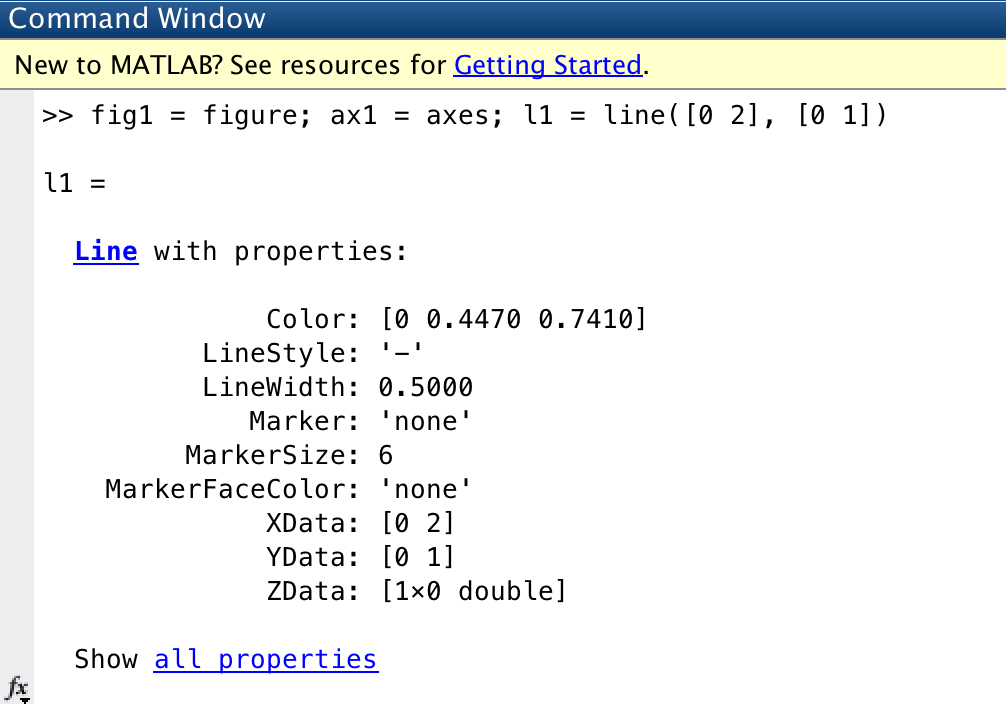
\includegraphics[width=0.475\textwidth]{graphics/NewFigAxLineCmdWinOut.png}
   \label{subfig:NewFigAxLineCmdWin}}
   \subfigure[ ]{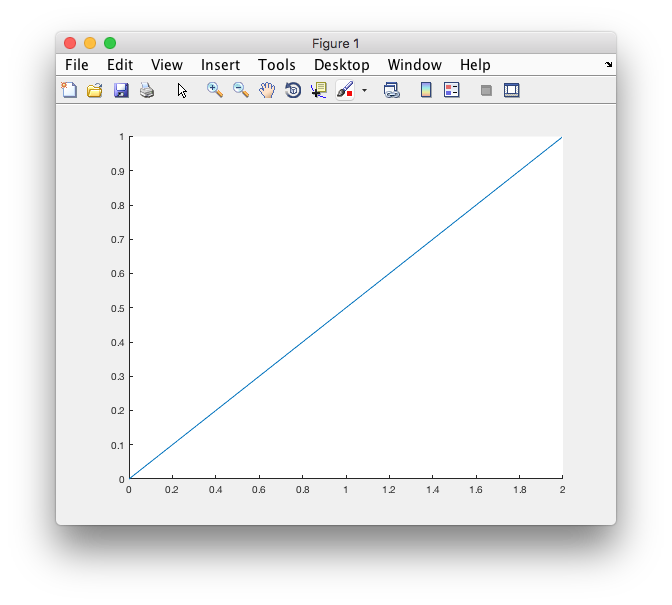
\includegraphics[width=0.475\textwidth]{graphics/NewFigAxLine.png} \label{subfig:NewFigAxLineWin}}
   \caption{Command Window output and graphical output of code of Listing \ref{NewFigAxLine}.}
   \label{fig:NewFigAxLine}
\end{figure}
% ^^^------------------------------------------------------------^^^
The \texttt{line} object \texttt{l1} has several properties, and many of these are suppressed in the Command Window output. Some important properties include \texttt{XData}, \texttt{YData}, \texttt{LineWidth}. Recall that we invoked the \texttt{line} constructor using \verb!line([0 2], [0 1])!. The first input array was a set of $x$-points and was stored in \texttt{l1.XData}. The second input array was a set of $y$-values, stored in \texttt{l1.YData}. Thus, the defining points for the \texttt{line} \texttt{l1} are given by making $(x,y)$ pairs from the values stored in these fields, and the line goes from $\mbox{(\texttt{XData(1)}, \texttt{YData(1)})}=(0,0)$ to $\mbox{(\texttt{XData(2)}, \texttt{YData(2)})}=(2,1)$.

% ============================================================
% ============================================================
\subsection{The Current \texttt{figure} and Current \texttt{axes} Objects}
% ============================================================
% ============================================================
Since \texttt{fig1} is the most recently-created \texttt{figure} object, it is referenced in MATLAB as the current figure. We can refer to it by the handle we created, \texttt{fig1}, or by the function \texttt{gcf} (get current figure), which returns a handle to the current \texttt{figure}. Similarly, \texttt{ax1} is the current \texttt{axes} object, which also may be referenced using \texttt{gca} (get current axes) or by \texttt{ax1}.

We can use the command \texttt{grid on} to toggle on grid lines for the current \texttt{axes}. Similarly, we can issue new plot commands, and they will generate new graphics objects as children of the current axes. We also can add $x$-axis and $y$-axis labels to the current \texttt{axes} by using the \texttt{xlabel} and \texttt{ylabel}. For example, consider Listing \ref{NewFigAxLinev01}:
% vvv------------------------------------------------------------vvv
\begin{lstlisting}[style=Matlab-editor,label=NewFigAxLinev01,caption={Command Window input to modify the \texttt{ax1}, the current axes object.}]
>> grid on; ax1.FontSize=16; xlbl = xlabel('$x$ (m)');  ylbl = ylabel('$y$ (m)'); xlbl.Interpreter='latex'; ylbl.Interpreter='latex';
\end{lstlisting}
% ^^^------------------------------------------------------------^^^
First, this input instructs MATLAB to display the grid; then, we enlarge the font for \texttt{ax1}; next, we define a variable \texttt{xlbl} as a handle for the \texttt{xlabel} object, which is assigned as a child of \texttt{ax1}. Similarly, \texttt{ylbl} is a handle for the \texttt{ylabel} object (also a child of \texttt{ax1}). The strings we provided within the \texttt{xlabel()} and \texttt{ylabel()} constructor methods enclose a symbol in dollar signs (\verb!$!). This is a fancy technique to make text appear as a mathematical expression as typeset in many textbooks. In order for this to work correctly, the appropriate object must have as it \texttt{Interpreter} property set to the value \texttt{'latex'}. We accomplish this is the remainder of the command in Listing \ref{NewFigAxLinev01}. The graphical result of Listing \ref{NewFigAxLinev01} is shown in Fig.\ \ref{subfig:NewFigAxLineWinv01}.
% vvv------------------------------------------------------------vvv
\begin{figure}[htbp] %  figure placement: here, top, bottom, or page
   \centering
   \subfigure[ ]{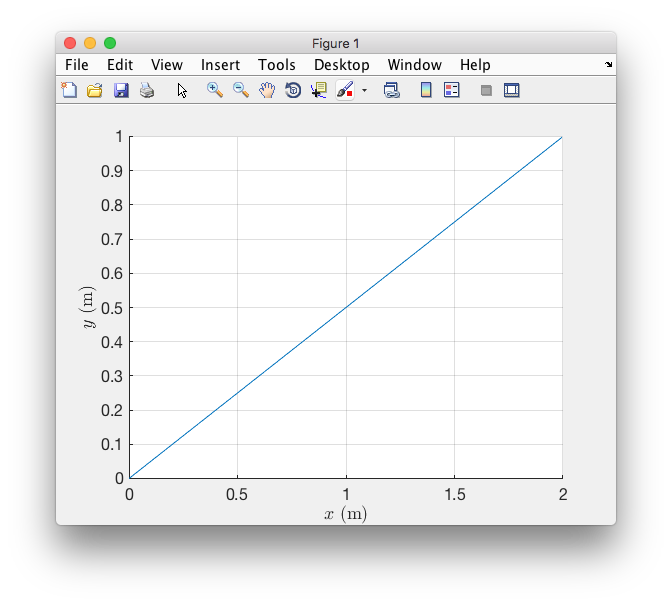
\includegraphics[width=0.475\textwidth]{graphics/NewFigAxLinev01.png} \label{subfig:NewFigAxLineWinv01}}
   \subfigure[ ]{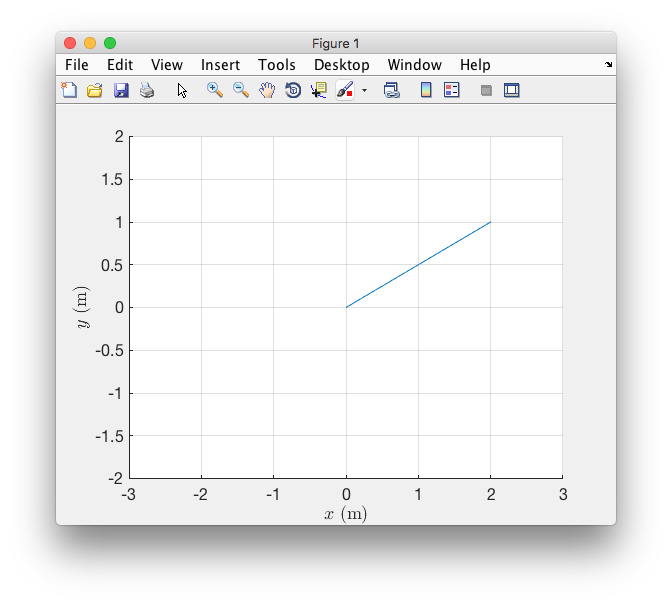
\includegraphics[width=0.475\textwidth]{graphics/NewFigAxLinev02axLims.png} \label{subfig:NewFigAxLineWinv02ScaledAx}}
   \caption{Command Window output and graphical output of code of Listing \ref{NewFigAxLine} [subfigure (a)] and Listing \ref{NewFigAxLinev01} [subfigure (b)]. In \ref{subfig:NewFigAxLineWinv01}, we have added a grid and axes labels. In \ref{subfig:NewFigAxLineWinv02ScaledAx}, we have adjusted the axes limits.}
   \label{fig:NewFigAxLine}
\end{figure}
% ^^^------------------------------------------------------------^^^
Compare Figs.\ \ref{subfig:NewFigAxLineWin} and \ref{subfig:NewFigAxLineWinv01} to see how we modified \texttt{ax1}.

% ============================================================
\subsubsection{Adjusting the Limits of the Current \texttt{axes}}
% ============================================================
It often is helpful to adjust the $x$- and $y$-limits of the current \texttt{axes}.  To do this, we can use the \texttt{xlim()} and \texttt{ylim()} functions. When invoked with no arguments, these functions return (get) a $1\times2$ array describing the $x$- or $y$-limits, but when invoked with a single $1\times2$ vector of the form \verb![vlo vhi]!, these functions set the applicable axes limits.
As an example, we set the axes limits to be $[-3, 3]$ in the $x$-direction and $[-2, 2]$ in the $y$-direction using the following command:
% vvv------------------------------------------------------------vvv
\begin{lstlisting}[style=Matlab-editor,label=NewFigAxLinevSetAxLim,caption={A Command Window input to set the axes limits for the current \texttt{axes} object.}]
>> xlim([-3 3]); ylim([-2 2])
\end{lstlisting}
% ^^^------------------------------------------------------------^^^
This creates a larger graphical context for the line segment we drew, as shown in Fig.\ \ref {subfig:NewFigAxLineWinv02ScaledAx}.

% ============================================================
% ============================================================
\subsection{Some Basic Graphic Types}
% ============================================================
% ============================================================

% ============================================================
\subsubsection{The \texttt{line} Class}
% ============================================================

We already have seen the \texttt{line} class, which we instantiated using the \texttt{line()} constructor method. To modify the line's end points, we can simply modify the \texttt{line} object's \texttt{XData} and \texttt{YData} properties. As an example, we can create a line using a script such as this \texttt{basicLine.m} script:
% vvv------------------------------------------------------------vvv
\begin{lstlisting}[style=Matlab-editor,label=basicLine,caption={Listing of the script \texttt{basicLine.m}.}]
% basicLine.m

a = 1; b = 2; c = 3; d = 4;
L0 = line([a b], [c d], 'LineWidth', 2);
\end{lstlisting}
% ^^^------------------------------------------------------------^^^
Upon running this script, we will have the \texttt{line} object \texttt{L0} saved in memory, and it can easily be seen that the \texttt{XData} property stores the vector \verb![1, 2]!, and that \texttt{YData} stores the vector \verb![3, 4]!,
% vvv------------------------------------------------------------vvv
\begin{lstlisting}[style=Matlab-editor,label=basicLineCheck,caption={A Command Window verification of the \texttt{XData} and \texttt{YData} properties of the \texttt{L0} object created in Listing \ref{basicLine}.}]
>> L0.XData

ans =

     1     2

>> L0.YData

ans =

     3     4
\end{lstlisting}
% ^^^------------------------------------------------------------^^^

Also, we can use the \texttt{plot()} command to specify \texttt{line} objects with two endpoints and many connected data points. To learn the syntax of the \texttt{plot()} command, either do an Internet search, or type \verb!doc plot! or \verb!help plot! in the MATLAB Command Window.

We can make several modifications to the \texttt{line} object by changing its properties. We list some important properties here:
\begin{itemize}
\item \texttt{XData}, \texttt{YData}, and \texttt{ZData} can be modified to change a 2D or 3D line object (yes, MATLAB can make 3D plots).
\item \texttt{LineWidth} can be used to change the thickness of the line.
\item \texttt{LineStyle} can be used to set the style of the line.
\item \texttt{Marker} can be used to specify a marker for data points.
\end{itemize}
To learn about the many options available to you, type \verb!doc line!.

% ============================================================
\subsubsection{The \texttt{patch} Class}
% ============================================================
A MATLAB \texttt{patch} draws a closed polygon with straight edges. The polygon is specified by specifying the $x$-, $y$-, and optional $z$ values of each vertex. The polygon is closed by connecting the last vertex to the first.

The basic syntax for the \texttt{patch} constructor is \texttt{patch(X,Y,C)}. This creates a polygon of $N$ points, where \texttt{X} is a $1\times N$ vector of $x$ values, $Y$ is a $1\times N$ vector of $y$ values, and \texttt{C} is a color specifier. The color specifier can be a string to specify a basic color, such as \verb!'r'!, \verb!'g'!,\verb!'b'!,\verb!'c'!,\verb!'m'!,\verb!'y'!,\verb!'w'!, or \verb!'k'!; or, \texttt{C} may be a $3$-element RGB (red-blue-green) triple specifying an arbitrary color. For example: \verb!C = [1, 0, 0]! specifies elementary red; \verb!C = [0, 1, 0]! specifies green; \verb!C = [0, 0, 1]! specifies blue; \verb!C = [0, 0, 0]! specifies black; and \verb!C = [1, 1, 1]! specifies white.

As an example, I provide the listing of a \texttt{basicPatch.m} script. The patch is defined in lines 3-7, and following lines of code provide formatting.
% vvv------------------------------------------------------------vvv
\begin{lstlisting}[style=Matlab-editor,label=basicPatch,caption={Listing of the script \texttt{basicPatch.m}.}]
% basicPatch.m

x = [-1 -1 1 1]; % specify x-values for vertices
y = [-1 1 1 -1]; % specify y-values for vertices
C = [0.75 0 0.75]; % specify a purple-ish color

newSquare = patch(x, y, C)
set(gca, 'FontName', 'Times', 'FontSize', 20); % format the current axes
grid on;

xlim([-3 3]); % adjust the x-limits of the axis
ylim([-3 3]); % adjust the x-limits of the axis

xlabel('$x$ (m)', 'Interpreter', 'latex') % add an x-label
ylabel('$y$ (m)', 'Interpreter', 'latex') % add a y-label
\end{lstlisting}
% ^^^------------------------------------------------------------^^^
The output of the \texttt{basicPatch.m} script is shown in Fig.\ \ref{fig:basicPatchOutput}.

% vvv------------------------------------------------------------vvv
\begin{figure}[htbp] %  figure placement: here, top, bottom, or page
   \centering
   \subfigure[ ]{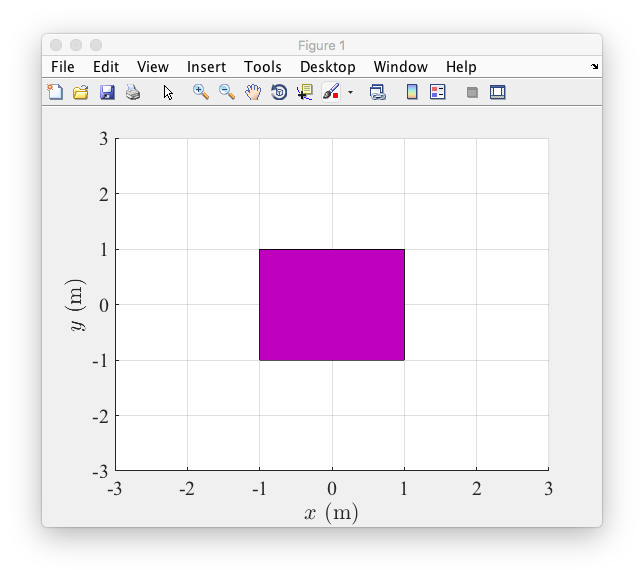
\includegraphics[width=0.475\textwidth]{graphics/basicPatchOutGraphical.png} \label{subfig:basicPatchOutputGraph}}
   \subfigure[ ]{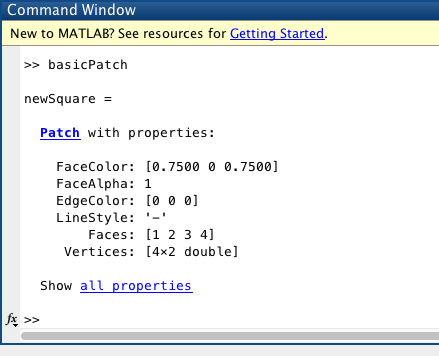
\includegraphics[width=0.475\textwidth]{graphics/basicPatchOutText.png} \label{subfig:basicPatchOutputText}}
   \caption{Graphical and Command Window output of the \texttt{basicPatch.m} script of Listing \ref{basicPatch}.}
   \label{fig:basicPatchOutput}
\end{figure}
% ^^^------------------------------------------------------------^^^

%The unsupressed output of Line 7 lists some properties of the \texttt{patch} object.
The \texttt{patch} object is centered at the origin in Fig.\ \ref{subfig:basicPatchOutputGraph}. An example of a simple modification to this is to translate the patch by the vector $(\Delta x, \Delta y)$. To do this, we define $\Delta x$ and $\Delta y$, and add these to the original \texttt{XData} and \texttt{YData} properties of the \texttt{newSquare} object. This can be done in the Command Window using the \texttt{set()} function:
% vvv------------------------------------------------------------vvv
\begin{lstlisting}[style=Matlab-editor,label=basicPatchDisplace,caption={A Command Window modification to the \texttt{patch} defined in Listing \ref{basicPatch}. Line 1 is used to specify the $x$- and $y$-components of the displacement. The displacement is then applied to the original \texttt{XData} and \texttt{YData} properties, and the result of the addition is the value component of a property-value pair in the \texttt{set()} function.}]
>> Dx = -2; Dy = 1.5;
>> set(newSquare, 'XData', newSquare.XData + Dx, 'YData', newSquare.YData + DY)
\end{lstlisting}
% ^^^------------------------------------------------------------^^^
The syntax here is \verb!set(obj, Prop1, Val1, Prop2, Val2, ...)!, where \texttt{obj} is the object we wish to modify, and we use property-value pairs to assign new object properties. The displaced \texttt{patch} object is displayed in Fig.\ \ref{fig:basicPatchDisplaced}. Similar modifications may be made to a \texttt{line}-class object.

% vvv------------------------------------------------------------vvv
\begin{figure}[htbp] %  figure placement: here, top, bottom, or page
   \centering
   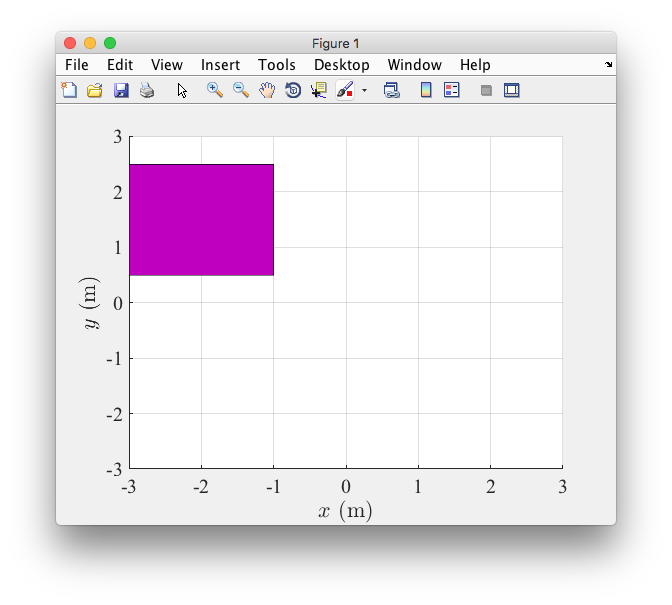
\includegraphics[width=0.475\textwidth]{graphics/basicPatchDisplaced.png}   
      \caption{The \texttt{patch} object created using \texttt{basicPatch.m} is modified by using the \texttt{set()} function using the code of Listing \ref{basicPatchDisplace}. The resulting \texttt{patch} no longer sits at the origin.}
\label{fig:basicPatchDisplaced}

\end{figure}
% ^^^------------------------------------------------------------^^^

For more information about the \texttt{patch} class, type \texttt{doc patch} in the MATLAB Command Window, or do an Internet search.
\section{Extended Example: Class Infrastructure for a Multi-player Game}

In this example, we develop some classes that may support a multi-player game, and we apply some visualization concepts in drawing a rudimentary game arena with avatars representing players. Therefore, we begin by defining an \texttt{Avatar} class. The example will continue with visualization of multiple avatars within a single \texttt{axes} object.

\subsection{Defining an \texttt{Avatar} Class}

We show a rudimentary \texttt{Avatar} class definition in Listing \ref{AvatarClassDef0}. Properties typical of a player's digital representation in a role-playing video game are present. The constructor method allows several different invocation syntaxes. Also, we have defined a \texttt{move()} method, which is used to change the \texttt{Avatar} object's position on the battlefield.
% vvv------------------------------------------------------------vvv
\begin{lstlisting}[style=Matlab-editor, label=AvatarClassDef0, caption={An initial class definition file for the \texttt{Avatar} class.}]
classdef Avatar
    %AVATAR objects represent a player in a multi-player role-playing game.
    %   The AVATAR class defines properties typical of avatars in RPGs.
    %
    % By E.P. Blair
    % Baylor University
    
    properties
        Name = 'Unidentified Player';
        Class % {'mage', 'warrior', 'thief', 'jedi', 'sith', 'none'}
        Level = 1; % a numerical rank for a player
        Position = [0 0]; % (x, y) double for
        XP = 0; % a numerical property for accumulating experience points
        HealthPointsMax = 100; % player's maximum health points (HP)
        Vitality = 1 % player's actual vitality (fraction of maximum vitality)
                     % HP = Vitality * HealthPointsMax
        Attack % numerical rating for offensive capabilities
        Defense % numerical rating for densive capabilities
        WeaponList % list of player's a offensive equipment
        ArmorList % list of player's a defensive equipment
        EquipmentList % list of player's equipment items
    end % END: properties
    
    methods
        function obj = Avatar(varargin)
            %Avatar instantiates an AVATAR object
            %   SYNTAX
            %
            %   newAvatar = Avatar creates a default AVATAR object
            %
            %   newAvatar = Avatar(Username) creates a default AVATAR
            %          object and specifies Username as the name.
            %
            %   newAvatar = Avatar(Username, PlayerClass) creates a default
            %           AVATAR object with name Username and class
            %           PlayerClass.
            %
            
            switch nargin
                case 0
                    obj.Class = 'none';
                case 1
                    obj.Name = varargin{1};
                    obj.Class = 'none';
                case 2
                    obj.Name = varargin{1};
                    obj.Class = varargin{2};
            end
        end
        
        function obj = move(obj, dispVect)
            % myPlayer = myPlayer.move( [dX dY] ) displaces the avatar on
            %   the battlefield.
            obj.Position = obj.Position + dispVect;
        end
        
        function disp(obj)
            % disp(someAvatar) is the display function for the AVATAR
            % class.
            disp([obj.Name, ' (Level ', num2str(obj.Level), ' ', ...
                obj.Class, ') is at (', ...
                num2str(obj.Position(1)) , ', ', ...
                num2str(obj.Position(2)), ').']);
        end
        
    end % END: methods
end
\end{lstlisting}
% ^^^------------------------------------------------------------^^^

\subsubsection{Overriding the \texttt{disp()} Function}
We also have defined a \texttt{disp()} function. Each bulit-in MATLAB class has its own particular \texttt{disp} function, which is invoked to display information about an object in question when an unsuppressed MATLAB calculation yields an object of that class. For a user-defined class, if no \texttt{disp()} method is defined, MATLAB displays that object in a manner similar to the display of a \texttt{struct}, giving a listing of all of the fields pertinent to that particular class. Here, we have a customized \texttt{disp()} method that is written to display the player's name, level and class, as well the battlefield position of the player's \texttt{Avatar} object. When a method \texttt{someMethod()} is defined for a class, but \texttt{someMethod()} already exists for other classes, we say that we have \textbf{overridden} the \texttt{someMethod()} method. Here, we have overridden the \texttt{disp} method to define a customized format for the display of information for objects of class \texttt{Avatar}.

As an example, see Listing \ref{AvatarClassDefTestCmdWin01}, where we test the new \texttt{Avatar} class definition in the Command Window. When the \texttt{Avatar} constructor is invoked (and not suppressed), the result is an object of class \texttt{Avatar}, so the \texttt{Avatar} class \texttt{disp()} method is invoked to display information about the resulting \texttt{Avatar} object:
% vvv------------------------------------------------------------vvv
\begin{lstlisting}[style=Matlab-editor, label=AvatarClassDefTestCmdWin01, caption={Command Window input and output to test the \texttt{Avatar} class constructor and overridden \texttt{disp()} method.}]
>> newAvatar = Avatar('Sargon', 'warrior')

newAvatar = 

Sargon (Level 1 warrior) is at (0, 0).
\end{lstlisting}
% ^^^------------------------------------------------------------^^^

\subsubsection{Testing the \texttt{move()} Method}
Next, we test the \texttt{move()} method in the Command Window:
% vvv------------------------------------------------------------vvv
\begin{lstlisting}[style=Matlab-editor, label=AvatarClassDefTestCmdWin02, caption={The \texttt{Avatar} class \texttt{move()} method worked as desired in a Command Window test.}]
>> newAvatar = newAvatar.move([27, -126])

newAvatar = 

Sargon (Level 1 warrior) is at (27, -126).
\end{lstlisting}
% ^^^------------------------------------------------------------^^^

\subsection{Graphical Visualization for the \texttt{Avatar} Class}

This is where writing the \texttt{Avatar} class gets fun and challenging. First, we will add a \texttt{draw()} method which draws a graphical representation of an \texttt{Avatar} object on an axes. This calls for adding a property to the \texttt{Asset} class which stores a handle to the drawing. When the \texttt{draw()} method is invoked, it can then check to see if the \texttt{Avatar} object already has a drawing; if so, we need not draw it again. Then, we will upgrade the \texttt{move()} method so that it not only changes the \texttt{Position} property, but also updates the \texttt{Avatar} object's drawing, as applicable.

% ============================================
% ============================================
\subsection{The \texttt{Avatar} Class \texttt{draw()} Method}
% ============================================
% ============================================
Listing \ref{AvatarClassDef01} shows the new snippets of the \texttt{Avatar} class definition file.
% vvv------------------------------------------------------------vvv
\begin{lstlisting}[style=Matlab-editor, label=AvatarClassDef01, caption={A \texttt{draw()} method was added to the \texttt{Avatar} class.}]
classdef Avatar
    %AVATAR objects represent a player in a multi-player role-playing game.
    %   The AVATAR class defines properties typical of avatars in RPGs.
    %
    % By E.P. Blair
    % Baylor University
    
    properties
        
        <-- snip -->        

        % Graphics-related properties
        Drawing % A struct of handles to the drawing components
        
    end % END: properties
    
    methods

        <-- snip -->        
                
        function obj = draw(obj, varargin)
            
            % Default values 
            TargetAxes = [];
            % Override default values: parse varargin for property-value
            %   pairs
            
            args = varargin;
            while length(args) >= 2
                prop = args{1};
                val = args{2};
                args = args(3:end);
                
                switch prop
                    case 'Axes'
                        TargetAxes = val;
                    otherwise
                        error(['''', prop, ''' is an invalid ', ...
                            'property specifier.'])
                end % END switch prop
            end % END while length(args) >= 2 
            
            if isempty(obj.Drawing)
                
                % DRAW THE SQUARE (MAIN BODY)
                % Calculate relative points of corners
                x_rel = [-5 -5 5 5];
                y_rel = [-5 5 5 -5];
                % Calculate absolute points of corners
                x = obj.Position(1) + x_rel;
                y = obj.Position(2) + y_rel;
                % visualization
                Drawing.Body = patch(x, y, [1 1 1], ...
                    'EdgeColor', [0 0 0], 'LineWidth', 2);

                NameText = text(obj.Position(1), obj.Position(2), ...
                    obj.Name, 'FontName', 'Times', 'FontSize', 18, ...
                    'HorizontalAlignment', 'center', ...
                    'VerticalAlignment', 'bottom');
                
                % PLAYER INFO STRING
                % 'LVL. X C' (X = Level, C = Class)
                PlayerInfoStr = ['LVL. ', num2str(obj.Level), ' ', ...
                    upper(obj.Class(1:3))];
                xPInfoStr = obj.Position(1);
                yPInfoStr = obj.Position(2) + 4;
                PlayerInfoText = text(xPInfoStr, yPInfoStr, PlayerInfoStr, ...
                    'FontName', 'Times', 'FontSize', 14, ...
                    'HorizontalAlignment', 'center', ...
                    'VerticalAlignment', 'middle');
                
                
                % HEALTH BAR
                % Full health will span [-4, 4] (relative)
                % No health is a point at -4 (relative
                % Color will transition from [0 0.5 0] (green, full)
                % to [1 0 0] (red, empty)
                cHealthLine = [ 1-obj.Vitality, 0.75*obj.Vitality, 0];
                xHealthLine = obj.Position(1) + [-4, -4+8*obj.Vitality];
                yHealthLine = obj.Position(2) - [2 2];
                HealthLine = line( xHealthLine, yHealthLine, ...
                    'Color', cHealthLine, ...
                    'LineWidth', 5);

                % HEALTH STATUS STRING (HealthStr)
                % 'HP: XX/MAX'
                HealthStr = ['HP: ', ...
                    num2str(round(obj.Vitality*obj.HealthPointsMax)), ...
                    '/', num2str(obj.HealthPointsMax)];
                xHealthStr = obj.Position(1) + 4;
                yHealthStr = obj.Position(2) - 3.5;
                HealthText = text(xHealthStr, yHealthStr, HealthStr, ...
                    'FontName', 'Times', 'FontSize', 14, ...
                    'HorizontalAlignment', 'right', ...
                    'VerticalAlignment', 'middle');

                % Populate the Drawing struct
                Drawing.PlayerInfoText = PlayerInfoText;
                Drawing.HealthText = HealthText;
                Drawing.Health = HealthLine;
                
                % store Drawing in obj.Drawing
                obj.Drawing = Drawing;
                
            end
        end
        
    end % END: methods
end
\end{lstlisting}
% ^^^------------------------------------------------------------^^^
The \texttt{draw()} method provides some nice features here:
\begin{itemize}
\item \texttt{draw()} supports optional property-value pairs using \texttt{varargin}. A block is reserved for default values (lines 22-23), which then can be optionally overridden by using the property-value pairs (lines 28-41).
\item Line 43 is used to evaluate whether drawing is necessary. Drawing only commences if the \texttt{obj.Drawing} object is empty, which is the case for any newly-created \texttt{Avatar} object (see the newly-added \texttt{Drawing} property on line 13).
\item Drawing begins with a square patch of side length 10, centered at the \texttt{Avatar} object's position (lines 45-54).
\item \texttt{draw()} writes the character's name in the center of the square patch. See lines 56-59.
\item \texttt{draw()} provides a player information string, with character level and the first three letters of the character class. See lines 61-70.
\item A health bar is shown below the character name. Its length decreases as the character's vitality decreases from full health (\texttt{Vitality = 1}) to no health (\texttt{Vitality = 0}). Additionally, the health bar will turn red as \texttt{Vitality} approaches 0. See lines 73-83.
\item A health string is shown at the bottom, including the current number of health points and the maximum number of health points for the player (lines 85-96).
\end{itemize}

Thus, the result of the testbed function \texttt{testbedAvatar.m} (Listing \ref{AvatarDrawTestbed}) is the MATLAB \texttt{figure} shown in Fig.\ \ref{fig:AvatarDrawing}. At this point, the \texttt{draw()} method seems to work as well as designed. Next steps include:
\begin{itemize}
\item Upgrading the \texttt{move()} method to update the graphics objects stored within the \texttt{Drawing} property.
\item Adding functions such an \texttt{updateStatus()} method, which and update the data represented in the drawing. This method also could be called by other methods, such as \texttt{injure()} and \texttt{heal()}, which adjust the player's \texttt{Vitality} property, along with updating the drawing data.
\end{itemize}
% vvv------------------------------------------------------------vvv
\begin{lstlisting}[style=Matlab-editor, label=AvatarDrawTestbed, caption={A testbed function tests the new \texttt{draw()} method.}]
% testbedAvatar.m
close all;
clear all;

Player1 = Avatar('Sargon', 'warrior') % create Player1

Player1 = Player1.move([-3, 13]) % displace Player1

Player1 = Player1.draw; % execute draw()

xlim([-20, 20]); % adjust the x limits beyond the square patch
axis equal % make the x- and y-scales equal
\end{lstlisting}
% ^^^------------------------------------------------------------^^^

% vvv------------------------------------------------------------vvv
\begin{figure}[htbp] %  figure placement: here, top, bottom, or page
   \centering
   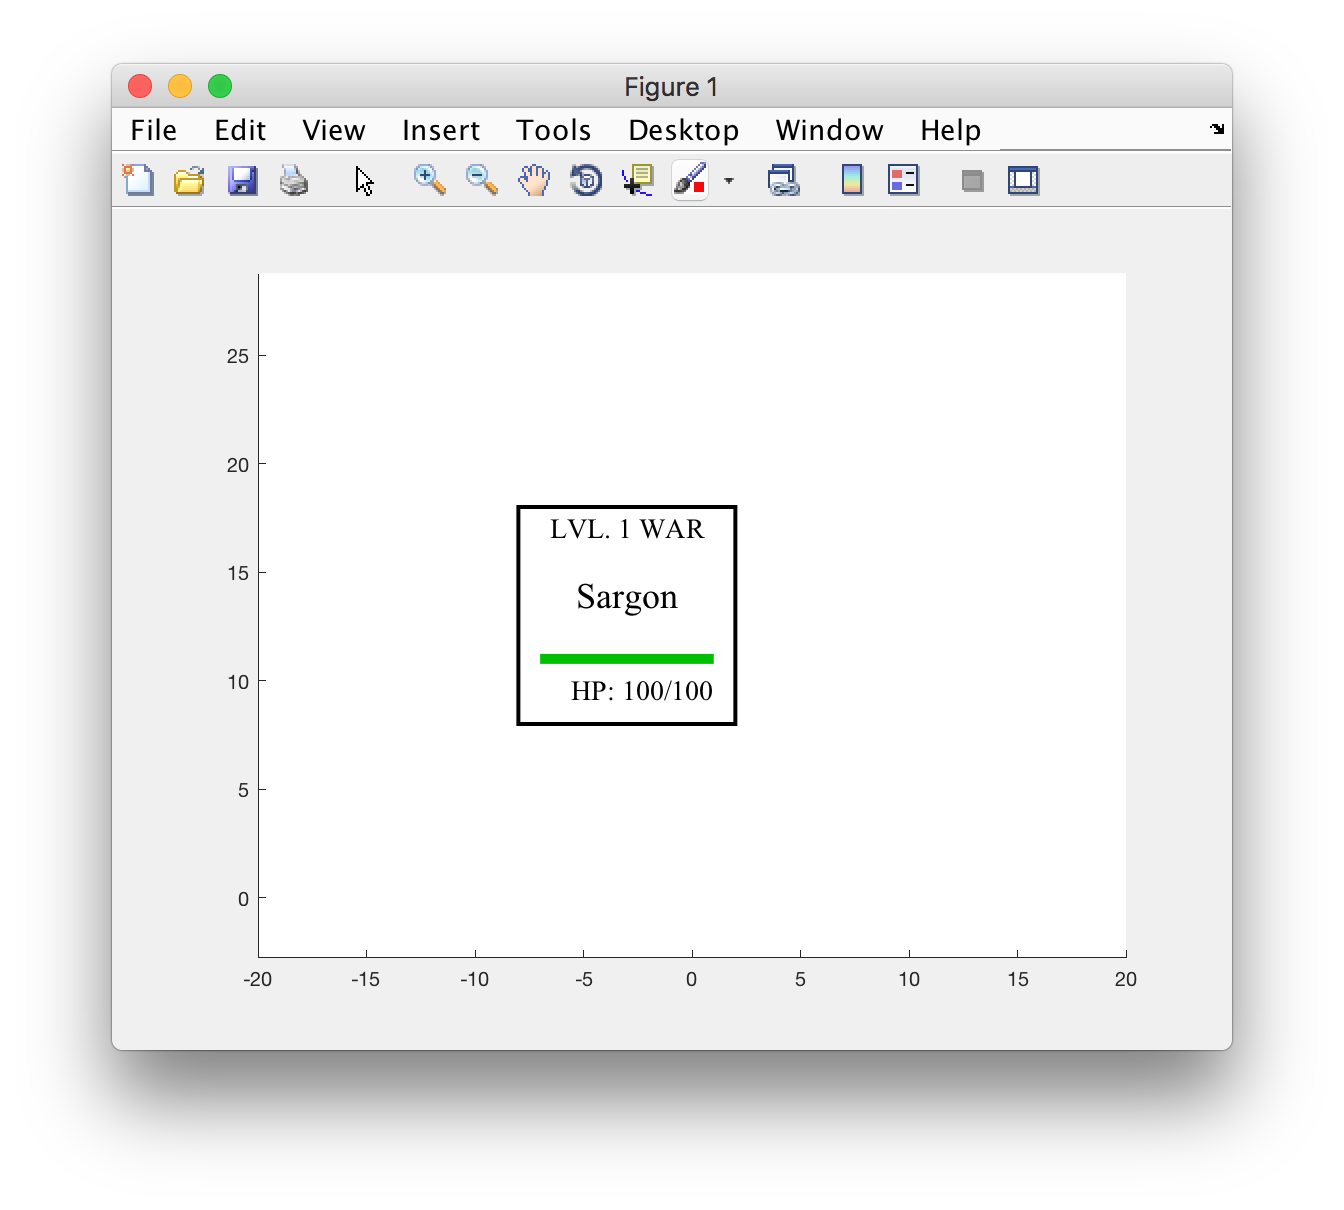
\includegraphics[width=5in]{graphics/AvatarDrawGraphOut.png} 
   \caption{A rudimentary graphical representation for an \texttt{Avatar} object. Here, \texttt{Player1} has the name \texttt{'Sargon'} and is drawn to indicate level 1 status as a warrior with full health (100/100 HP).}
   \label{fig:AvatarDrawing}
\end{figure}
% ^^^------------------------------------------------------------^^^
\appendix

% ============================================================
% ============================================================
% ============================================================
\section{Control Statements}
% ============================================================
% ============================================================
% ============================================================


% ============================================================
% ============================================================
\subsection{\texttt{if}-\texttt{elseif}-\texttt{else}-\texttt{end}}
% ============================================================
% ============================================================
Perhaps the simplest control statement is the achieved using \texttt{if}-\texttt{elseif}-\texttt{else}-\texttt{end}. The simplest version of this is an \texttt{if}-\texttt{end} statement, with the following typical syntax in a script or function:
% vvv------------------------------------------------------------vvv
\begin{lstlisting}[style=Matlab-editor]
if ctrl_expr
	statements
end
\end{lstlisting}
% ^^^------------------------------------------------------------^^^
Here, the control begins with \verb!if ctrl_expr! and ends with the key word \texttt{end}. The statements are executed if the real part of the control expression \verb!ctrl_expr! has all non-zero elements.

Most typically, \verb!ctrl_expr! is an expression which evaluates to a \texttt{logical} or a \texttt{double} value. An example of this is
% vvv------------------------------------------------------------vvv
\begin{lstlisting}[style=Matlab-editor]
% basic_if_control.m

a = true
if a
    disp('''a'' is true.')
end
\end{lstlisting}
% ^^^------------------------------------------------------------^^^
The output of \verb!basic_if_control.m! is
% vvv------------------------------------------------------------vvv
\begin{lstlisting}[style=Matlab-editor]
>> basic_if_control

a =

  logical

   1

'a' is true.
\end{lstlisting}
% ^^^------------------------------------------------------------^^^
Notice that \texttt{a} is a logical value, and it results in the execution of the block within the \texttt{if}-\texttt{end} construct.

Optionally, the \texttt{else} key word adds a section which is executed if the preceding sections of the \texttt{if} control is not executed. The \texttt{if}-\texttt{else}-\texttt{end} syntax is demonstrated as follows.

As an example of this, consider the function \verb!sign_fun()!:
% vvv------------------------------------------------------------vvv
\begin{lstlisting}[style=Matlab-editor]
function sign_fun(x)
% sign_fun(x) prints a message about the negativity of x.
%
% By E.P. Blair
% Baylor University

if x < 0
    disp('x is negative.')
else
    disp('x is non-negative.')
end
\end{lstlisting}
% ^^^------------------------------------------------------------^^^
This function was invoked on the command line with several test inputs:
% vvv------------------------------------------------------------vvv
\begin{lstlisting}[style=Matlab-editor]
>> sign_fun(-5)
x is negative.
>> sign_fun(-1.25)
x is negative.
>> sign_fun(0)
x is non-negative.
>> sign_fun(1)
x is non-negative.
>> 
\end{lstlisting}
% ^^^------------------------------------------------------------^^^

The \texttt{if}-\texttt{else}-\texttt{end} syntax allows for two different outcomes. Optional \texttt{elseif} blocks may be added to support additional possible outcomes. Consider, for example, this improved version of \verb!sign_fun()!:
% vvv------------------------------------------------------------vvv
\begin{lstlisting}[style=Matlab-editor]
function sign_fun(x)
% sign_fun(x) prints a message about the sign of x.
%
% By E.P. Blair
% Baylor University

if x < 0
    disp('x is negative.')
elseif x > 0
    disp('x is positive.')
else
    disp('x is zero.')
end
\end{lstlisting}
% ^^^------------------------------------------------------------^^^
The command line inputs and outputs for several tests are shown below.
% vvv------------------------------------------------------------vvv
\begin{lstlisting}[style=Matlab-editor]
>> sign_fun(-2)
x is negative.
>> sign_fun(3)
x is positive.
>> sign_fun(0)
x is zero.
\end{lstlisting}
% ^^^------------------------------------------------------------^^^

Multiple \texttt{elseif} blocks may be added, as in the following function, which assigns a letter grade given a percentage score:
% vvv------------------------------------------------------------vvv
\begin{lstlisting}[style=Matlab-editor]
function lg = letter_grade(percentScore)
% letter_grade maps a percentage score to a letter grade.

if percentScore < 60
    lg = 'F';
elseif percentScore < 70
    lg = 'D';
elseif percentScore < 80
    lg = 'C';
elseif percentScore < 90
    lg = 'B';
else
    lg = 'A';
end
\end{lstlisting}
% ^^^------------------------------------------------------------^^^

% ============================================================
% ============================================================
% ============================================================
\subsection{\texttt{for} Loops}
% ============================================================
% ============================================================
% ============================================================

% ============================================================
% ============================================================
% ============================================================
\subsection{\texttt{switch}-\texttt{case} Controls} \label{appendix:switch_case}
% ============================================================
% ============================================================
% ============================================================

A \texttt{switch}-\texttt{case} is useful when a finite, discrete set of cases may occur. The syntax for a \texttt{switch}-\texttt{case} control is as follows:
% vvv------------------------------------------------------------vvv
\begin{lstlisting}[style=Matlab-editor]
switch expr
	case expr_1
		statement_group_1
	case expr_2
		statement_group_2
	...
	otherwise
		statement_group_otherwise
end
\end{lstlisting}
% ^^^------------------------------------------------------------^^^
Here, the controlling expression evaluates to either a \texttt{char} string or an integer. If \texttt{expr} matches \verb!expr_1!, then only \verb!statement_group_1! executes; if \texttt{expr} matches \verb!expr_2!, then only \verb!statement_group_2! executes. The \texttt{otherwise} key word defines another block of statements that executes if \texttt{expr} does not match any of the expressions following a \texttt{case} key word. \texttt{Asset/calculateValue()} avoids the calculation if the \texttt{Asset} object's \texttt{transactionList} property is empty by using an \verb!if ~isempty(obj.transactionList)! block. Thus, the block executes if \texttt{obj.transactionList} is not empty. Inside this block, a \texttt{for} loop iterates through each transaction and calculates/records the number of units transacted. \texttt{Asset/calculateValue()} uses a the price-per-unit data to determine the transaction cost, the total value, and the cost basis for the asset holdings.

 


% ============================================
% ============================================
% ============================================
% ============================================
% ============================================
% ============================================
\end{document}
% ============================================
% ============================================
% ============================================
% ============================================
% ============================================
% ============================================


